% TODO: standardized equation notation. Is it eqn, Eqn, Eq? (all three are used).



\chapter{Allele and Genotype Frequencies}
 In this chapter we will
work through how the basics of Mendelian genetics play out at the population
level in sexually reproducing organisms.

	Loci and alleles are the basic currency of population genetics--and indeed of
genetics. \marginnote[-1cm]{A
\emph{locus} (plural: \emph{loci}) is a specific spot in the
genome. The term allele was coined by
\href{https://en.wikipedia.org/wiki/Edith_Rebecca_Saunders}{Edith
  Rebecca Saunders} and  William Bateson in 1902 in their paper ``The facts of heredity in the light of Mendel’s discovery'' .} A locus
may be an entire gene, or a single nucleotide base pair such as A-T. At each
locus, there may be multiple genetic variants segregating in the
population---these different genetic variants are known as \emph{alleles}. If
all individuals in the population carry the same allele, we say that the locus
is \emph{monomorphic}; at this locus there is no genetic variability in the
population. If there are multiple alleles in the population at a locus, we say
that this locus is \emph{polymorphic} (this is sometimes referred to
as a segregating site).

\begin{marginfigure}[3cm]
\begin{center}
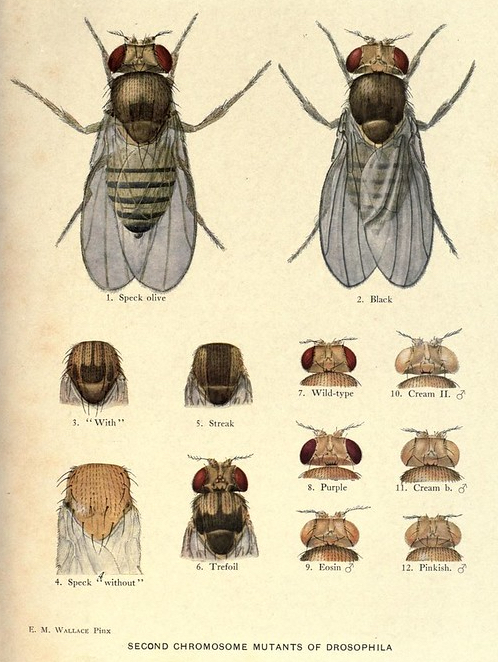
\includegraphics[width= 0.8 \textwidth]{illustration_images/alleles_genotypes/Drosophila_mel/Drosophila_mel_mutants.jpg}
\end{center}
\caption{ {\it Drosophila melanogaster} holds a special place in the
  history of genetics and population genetics. From Morgan's fly room discovering the principals of genetics to Dobzhansky's early work
  on natural genetic variation.  \BHLNC{Contributions to the genetics of Drosophila melanogaster
    (1919). Morgan T.H., Bridges C.B., Sturtevant A. H.}{https://www.biodiversitylibrary.org/page/805594\#page/147/mode/1up}{MBLWHOI Library} } \label{fig:dros}
\end{marginfigure}



Table \ref{Table:ADH} shows a small stretch of orthologous sequence for
the ADH locus from samples from {\it Drosophila melanogaster},  {\it D. simulans},
and {\it D. yakuba}.  {\it D. melanogaster} and {\it D. simulans} are
sister species and  {\it D. yakuba} is a close outgroup to the two.  Each column represents a single haplotype from an
individual (the individuals are diploid but were inbred so they're
homozygous for their haplotype). Only sites that differ among
individuals of the three species are shown. Site $834$ is an example
of a polymorphism; some  {\it D. simulans} individuals carry a $C$
allele while others have a $T$. \emph{Fixed differences}  are sites that differ between the species but are monomorphic within
  the species. Site $781$ is an example of a fixed difference between
  {\it D. melanogaster} and the other two species.

We can also annotate the alleles and loci in various ways. For example, position
$781$ is a non-synonymous fixed difference. We call the less common
allele at a polymorphism the  \emph{minor allele} and the common
allele the \emph{major allele}, e.g. at site $1068$ the $T$ allele is the
minor allele in {\it D. melanogaster}. We call the more evolutionarily
recent of the two alleles the \emph{derived allele} and the older of
the two the \emph{ancestral allele}. We infer that the $T$ allele at site 1068 is
the derived allele because the $C$ is found in both other species,
suggesting that the $T$ allele arose via a $C \rightarrow T$ mutation.

% For example, at a particular nucleotide site in the genome, a population may segregate for A-T and G-C base pairs (note that due to the complementary nature of DNA, it will suffice to say the site segregates for A and G variants).

\begin{table*}
  \tiny
\setlength{\tabcolsep}{.45\tabcolsep}   % https://tex.stackexchange.com/questions/307770/centered-tabular-column-with-narrow-columns
 %\csvreader[tabular=c]{Journal_figs/alleles_genotypes/ADH_MK/ADH.csv}
\csvautobooktabular{Journal_figs/alleles_genotypes/ADH_MK/ADH.csv}  % can control this more https://mirror.hmc.edu/ctan/macros/latex/contrib/csvsimple/csvsimple.pdf
  \caption{Variable sites in exons 2 and 3 of the ADH gene in {\it Drosophila} \citet{mcdonald:91}.
The first column (pos.) gives the position in the gene; exon 2 begins at
position $778$ and we've truncated the dataset at site $1175$.
The second column gives the consensus nucleotide (con.), i.e. the most
common base at that position; individuals with nucleotides that match
the consensus are marked with a dash.  The first columns of sequence
(a-l) are from {\it D. melanogaster};
    the next columns (a-f) give sequences from \textit{D. simulans}, and the final
 set of columns (a-l ) from {\it D. yakuba}. The last column shows
 whether the difference is a non-synonymous (N) or synonymous (S) change. }  % I've dropped the
                                % heterozygote sites from D. yakuba.
  \label{Table:ADH}
\end{table*}

\begin{question}
{\bf A)} How many segregating sites does the sample from \textit{
  D. simulans} have in the ADH gene?\\
{\bf B)} How many fixed differences are there between \textit{D. melanogaster} and \textit{D. yakuba}?
%What is the per base divergence are there between {\emph D. melanogaster} and {\emph D. yakuba}?
\end{question}
%JRI: confusing because site 974 is tri-allelic so "fixed" for derived allele but...

\section{Allele frequencies}
Allele frequencies are a central unit of population genetics
analysis, but from diploid individuals we only get to observe genotype
counts. Our first task then is to calculate allele frequencies from
genotype counts. Consider a diploid autosomal locus segregating for two alleles ($A_1$ and
$A_2$). We'll use these arbitrary labels for our alleles, merely to keep this
general. Let $N_{11}$ and $N_{12}$ be the number of $A_1A_1$ homozygotes and
$A_1A_2$ heterozygotes, respectively. Moreover, let $N$ be the total number of
diploid individuals in the population. We can then define the relative
frequencies of $A_1A_1$ and $A_1A_2$ genotypes as $f_{11} = N_{11}/N$ and
$f_{12} = N_{12}/N$, respectively. The frequency of allele $A_1$ in the
population is then given by

\begin{equation}
  p = \frac{2 N_{11} + N_{12}}{2N} = f_{11} + \frac{1}{2} f_{12}.
\end{equation}
Note that this follows directly from how we count alleles given individuals'
genotypes, and holds independently of Hardy--Weinberg proportions and
equilibrium (discussed below). The frequency of the alternate allele ($A_2$) is
then just $q=1-p$.

\subsection{Measures of genetic variability}
\paragraph{Nucleotide diversity ($\pi$)}
One common measure of genetic diversity is the average number of single
nucleotide differences between haplotypes chosen at random from a
sample. This is called \emph{nucleotide diversity} and is often denoted by
$\pi$.
For example, we can calculate $\pi$ for our ADH locus from Table \ref{Table:ADH} above: we have
6 sequences from \textit{D. simulans}  (a-f), there's a total of 15 ways of pairing
these sequences, and
\begin{equation}
\pi=\frac{1}{15} \big( (2 + 1 + 1 + 1 + 0 ) + (3 + 3 + 3 + 2 ) +(0 + 0 + 1) + (0 + 1) + (1)  \big)=1.2\overline{6}
\end{equation}
where the first bracketed term gives the pairwise differences between
a and b-f, the second bracketed term the differences between b and c-f
and so on. \\

Our $\pi$ measure will depend on the length of sequence it is calculated
for. Therefore, $\pi$ is usually normalized by the length of sequence,
to be a per site (or per base) measure. For example, our ADH sequence covers $397$bp of DNA and so $\pi = 1.2\overline{6}/397=0.0032$ per site in \textit{D. simulans} for this region. Note that we could also calculate $\pi$ per synonymous site (or non-synonymous). For synonymous site $\pi$, we would count up number of synonymous differences between our pairs of sequences, and then divide by the total number of sites where a synonymous change could have occurred.{\sidenote{Technically we would need to divide by the total number of possible point mutations that would result in a synonymous change; this is because some mutational changes at a particular nucleotide will result in a non-synonymous or synonymous change depending on the base-pair change.}


\paragraph{Number of segregating sites.} Another measure of genetic variability is the total number of sites
that are polymorphic (segregating) in our sample. One issue is that
the number of segregating sites will grow as we sequence more
individuals (unlike $\pi$). Later in the course, we'll talk about how to standardize the
number of segregating sites for the number of individuals sequenced (see eqn \eqref{watterson_theta}).

\paragraph{The frequency spectrum.}
We also often want to compile information about the frequency of
alleles across sites.  We call alleles that are found once in a sample
\emph{singletons}, alleles that are found twice in a sample {\emph
  doubletons}, and so on. We count up the number of loci where an
allele is found $i$ times out of $n$, e.g. how many singletons are
there in the sample, and this is called the \emph{frequency
  spectrum}. We'll want to do this in some consistent manner, such as calculating the frequency spectrum of the minor allele or the derived allele.

\begin{question}
How many minor-allele singletons are there in \textit{D. simulans} in
the ADH region? [Defining minor allele just within \textit{D. simulans}.]
%JRI: ambiguous. is the minor allele defined across all species or just within simulans?
\erin{students were confused whether you are defining 'minor allele' with reference to the species or to the whole group. There are no major allele singletons with reference to the individual species, but I think it's confusing because the only example of a minor allele given in the text by its definition is the 'minor allele in D. melanogaster' .. maybe it would be best to clarify in the question or just give an example of the minor allele in the whole sample instead.}
 \end{question}
\paragraph{Levels of genetic variability across species.}
Two observations have puzzled population geneticists since the
inception of molecular population genetics. The first is the relatively high
level of genetic variation observed in most obligately sexual species.
This first observation, in part, drove the development of the Neutral
theory of molecular evolution, the idea that much of this molecular
polymorphism may simply reflect a balance between genetic drift and
mutation.
The second observation is the relatively narrow range of
polymorphism across species with vastly different census sizes. This
observation represented a puzzle as the Neutral theory predicts that
levels of genetic diversity should scale with population size. Much effort
in theoretical and empirical population genetics has been devoted to
trying to reconcile models with these various observations. We'll
return to discuss these ideas throughout our course.
%Neutral

\begin{marginfigure}[-1cm]
\begin{center}
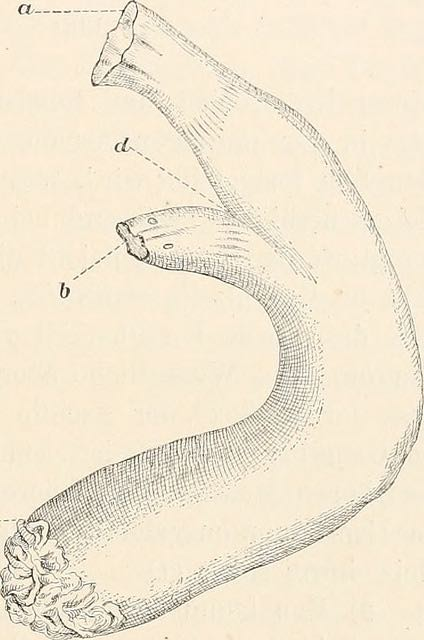
\includegraphics[width= 0.8 \textwidth]{illustration_images/alleles_genotypes/Ciona_intestinalis/21016139168_2a8a57ded3_z.jpg}
\end{center}
\caption{Sea Squirt ({\it Ciona intestinalis}). \BHLNKC{Einleitung in die vergleichende gehirnphysiologie und
  Vergleichende psychologie. Loeb, J. 1899.}{https://www.flickr.com/photos/internetarchivebookimages/21016139168/in/photolist-y28cZ3-xatkQu-w6Ki9C-wLcTJy-tLanR7-wKRZbh-w79C6u-toKNq1-u3ojn3-y8KsPP-xK7CZj-bu2usR-wLkfdM-wbkfau-x8n51o-ygpRAN-xMgGnk-towSTe-xQtix3-xMrift-wQoMNq-y51RxU-xPH4Cu-x4uB1v-xPGVFs-x4GN5a-y6rT8N-y6Aous-y7jV9n-yb6s66-x7F6Wh-y7upRp-xkz9VY-u1qerd-wYE4Cz-y5aH2Y-y7uJpM-xPSvFU-y6ALo7-xPZ3FM-xPHUef-yaa3dw-xPSKSC-w7A1aj-x4bgsH-tLas4q-x1e1dv-w7BkZB-xrQxFJ-y8acDr}{MBLWHOI Library}} \label{fig:ciona}
\end{marginfigure}

The first observations of molecular genetic diversity within natural populations were made from surveys of allozyme data, but we can revisit these general patterns with modern data. \\
\begin{figure*}
\begin{center}
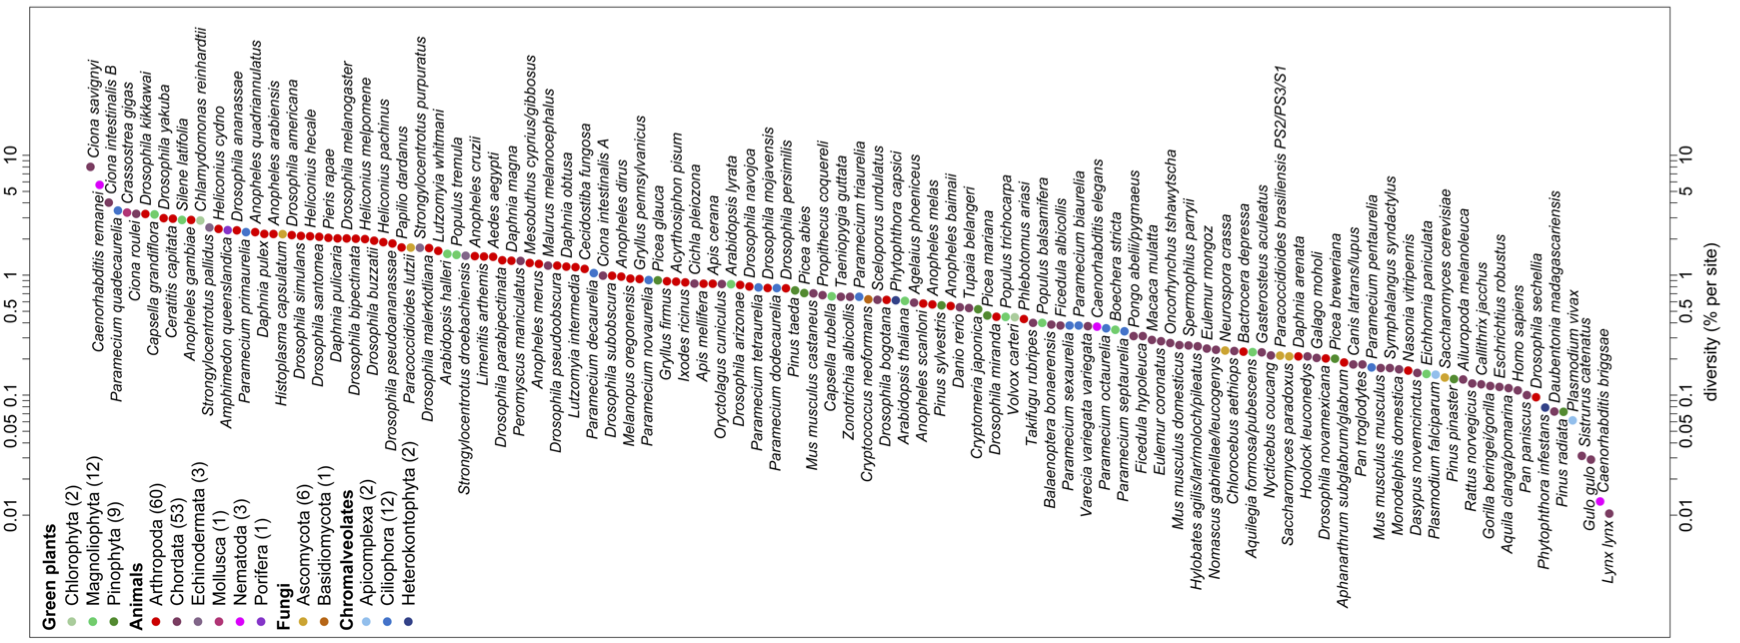
\includegraphics[width= \textwidth]{Journal_figs/alleles_genotypes/Leffer_riddle/Leffer_riddle_diversity.png}
\end{center}
\caption{Levels of autosomal nucleotide diversity for 167
species across 14 phyla. Figure 1 from \citet{leffler:12}, \PLOSccBY. Points are
ranked by their $\pi$, and coloured by their phylum. Note the log-scale.} \label{fig:Leffer}
\end{figure*}
For
example, \citet{leffler:12} compiled data on levels of within-population,
autosomal nucleotide diversity ($\pi$) for 167 species across 14 phyla from
non-coding and synonymous sites (Figure \ref{fig:Leffer}). The species with the lowest levels of
$\pi$ in their survey was Lynx, with $\pi = 0.01\%$, i.e. only
$1/10000$ bases differed between two sequences. In contrast, some of the highest levels of
diversity were found in {\textit{Ciona savignyi}, Sea Squirts, where a remarkable
$1/12$ bases differ between pairs of sequences. This $800$-fold range of
diversity seems impressive, but census population sizes have a much
larger range.
%JRI: I feel like an example of census size would be useful. the genus Cyclothone, which exists in the trillions, comes to mind as a surprising example that you could compare to like a coelocanth: https://commons.wikimedia.org/wiki/File:Wissenschaftliche_Ergebnisse_der_Deutschen_Tiefsee-Expedition_auf_dem_Dampfer_%22Valdivia%22_1898-1899_(Tafel_6)_(7413855904).jpg

\begin{marginfigure}[2cm]
\begin{center}
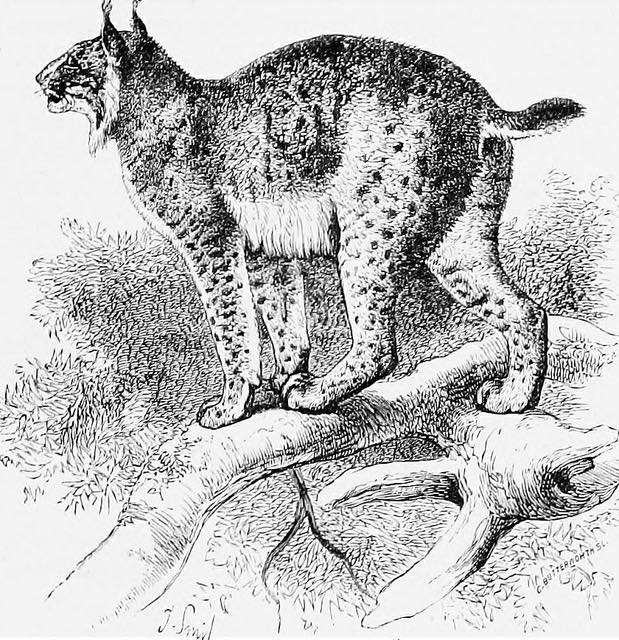
\includegraphics[width= 0.8 \textwidth]{illustration_images/alleles_genotypes/Lynx/20731949565_8a065700af_z.jpg}
\end{center}
\caption{Eurasian Lynx (\textit{Lynx lynx}). \BHLNKC{An introduction to the study
  of mammals living and extinct. Flower, W.H. and Lydekker, R. 1891.}{https://www.flickr.com/photos/internetarchivebookimages/20731949565/in/photolist-x5Jzv2-x6QVyp-xir9rH-wYHrQD-wPn1sP-w9PsqY-xDcqri-sMcQoB-trrkVd-x6Nx1H-wPea7N-sM28N9-tJ3zsp-xneVdx-wGJRtQ-xnfHZ8-wPfga7-xCUPrN-x7kXDV-xmAb9E-xm3x4k-xBoSKb-wGTgyB-xBoSbf-wGGvzA-xmzYTJ-oeKJcH-xA1Ffr-xA1Eji-xqWTQZ-xF4Lru-oxJfrH-x7ojSn-xra8zP-wGGibY-xgb21y-xY1jH9-xY1iyf-wGHxTS-wGQEoR-xmtPQh-x8uFKK-xdTkoU-wPggQf-wPfvHN-wPfc27-w9YnGF-wPeauS-wPiVxK-w6aiSi}{Cornell University Library}} \label{fig:Lynx}
\end{marginfigure}

\subsection{Hardy--Weinberg proportions}
Imagine a population mating at random with respect to genotypes, i.e. no
inbreeding, no assortative mating, no population structure, and no sex differences
in allele frequencies. The frequency of allele $A_1$ in the population at the
time of reproduction is $p$. An $A_1A_1$ genotype is made by reaching out into
our population and independently drawing two $A_1$ allele gametes to form a
zygote. Therefore, the probability that an individual is an $A_1A_1$ homozygote
is $p^2$. This probability is also the expected frequencies of the $A_1A_1$
homozygote in the population. The expected frequency of the three possible
genotypes are

\marginnote{Throughout this chapter we'll be making use of the basic
  rules of probability to find the probabilities of combinations of
  events, e.g. the alleles found in an individual, see Appendix \ref{Section_rules_prob} for a refresher.}

%\begin{table}[htp!]
\begin{center}
\begin{tabular}{ccc}
\hline
$f_{11}$ & $f_{12}$ & $f_{22}$ \\
\hline
$p^2$ & $2pq$ & $q^2$ \\
\end{tabular}
\end{center}
%\caption{\textbf{Hardy Weinberg}} \label{table:HWE}
%\end{table}
Note that we only need to assume random mating with respect to our focal allele in order for these expected frequencies to hold in the zygotes forming the next generation. Evolutionary forces, such as selection, change allele frequencies within generations, but do not change this expectation for new zygotes, as long as $p$ is the frequency of the $A_1$ allele in the population at the time when gametes fuse.
%\erin{I wasn't sure what contrast you were getting at here, so may not be a good edit}

\begin{question}
On the coastal islands of British Columbia there is a subspecies of
black bear (\textit{Ursus americanus kermodei}, Kermode's bear). Many members of this
black bear subspecies are white; they're sometimes called spirit bears. These
bears aren't hybrids with polar bears, nor are they albinos. They are
homozygotes for a recessive change at the MC1R gene. Individuals who
are $GG$ at this SNP are white while $AA$ and $AG$ individuals are black.



\begin{marginfigure}    %%%New Kermode_bear
                        %%%https://twitter.com/BioDivLibrary/status/1191354772034592774/photo/3
                        %%%page 77 https://www.biodiversitylibrary.org/item/38166?utm_source=Twitter&utm_medium=social+media&utm_term=&utm_content=MBLWHOI&utm_campaign=Mammal+Monday#page/114/mode/1up
  \begin{center}
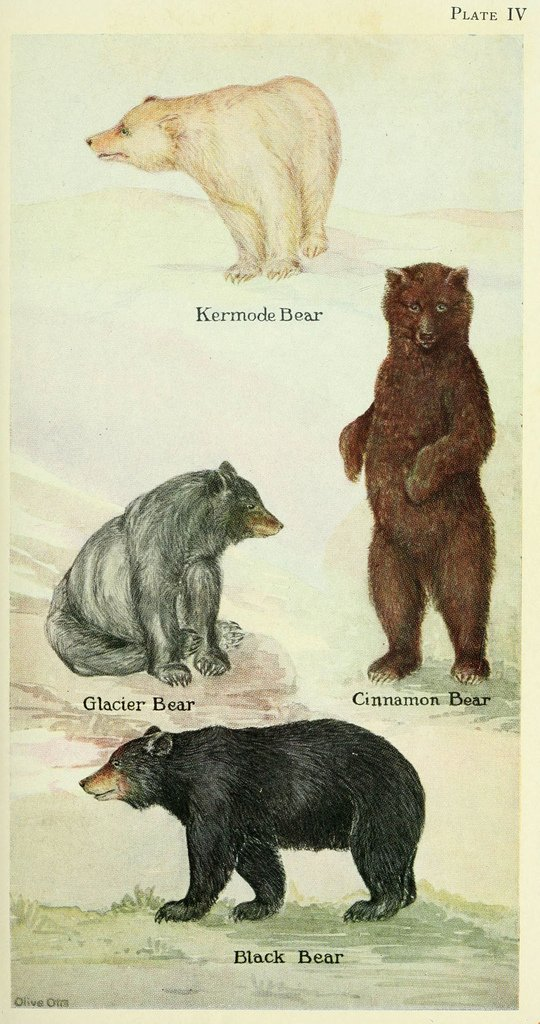
\includegraphics[width= \textwidth]{illustration_images/alleles_genotypes/Kermode_bear/EIiK2dsWoAAmUOf.jpeg}  
%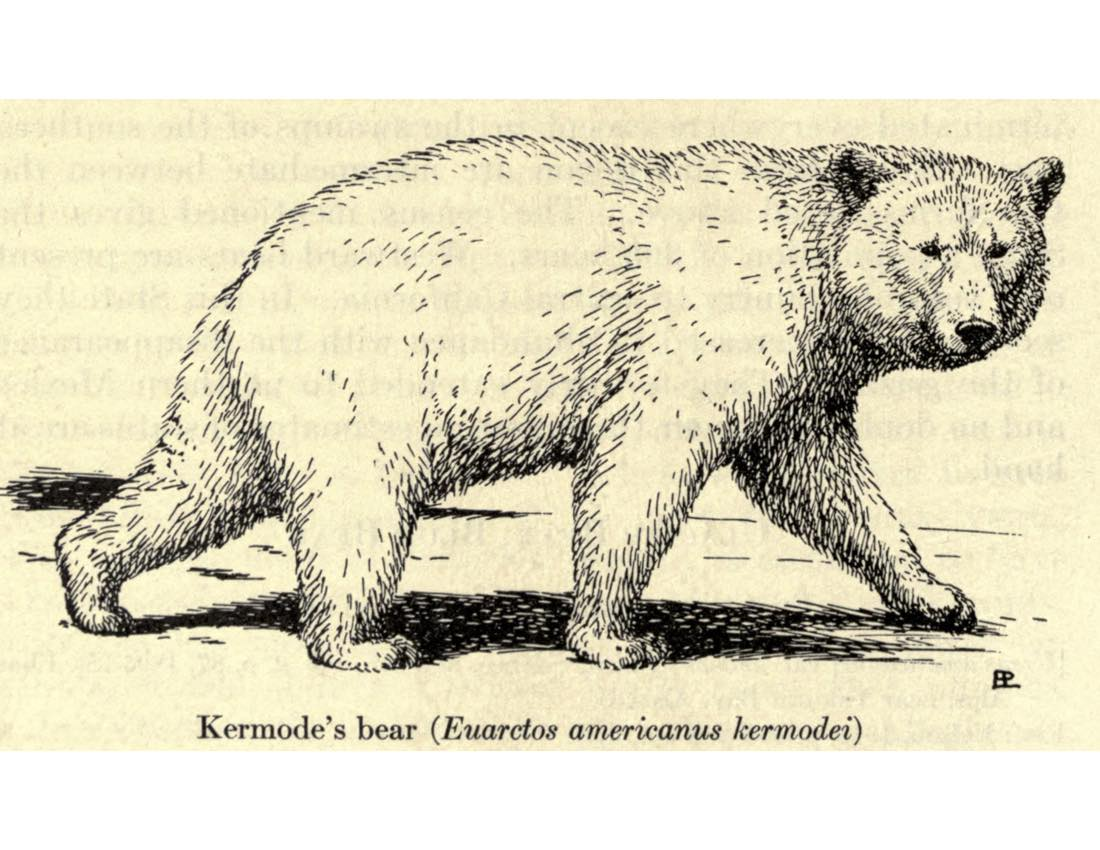
\includegraphics[width= \textwidth]{illustration_images/alleles_genotypes/Kermode_bear/Kermode_bear.jpg}
\end{center}
\caption{Kermode's bear (\textit{Ursus americanus kermodei}). It's
  possible that this morph is favoured as the salmon these bears eat have a harder time
  seeing the light morph \citep{klinka2009adaptive}. The adaptive
  value of tasting like cinnamon is unknown. \BHLNKC{Field book of North American mammals;
    descriptions of every mammal known north of the Rio
    Grande. Anthony, (1928) H. E.}{https://www.biodiversitylibrary.org/item/38166\#page/115/mode/1up}{MBLWHOI Library} } \label{fig:Kermodes_bear}
%\caption{Kermode's bear. \BHLNC{Extinct and vanishing mammals of the western
 % hemisphere. 1942. Glover A.}{https://www.biodiversitylibrary.org/page/20699033\#page/160/mode/1up}{Prelinger
%  Library} } \label{fig:Kermodes_bear}
\end{marginfigure}

Below are the genotype counts for the MC1R polymorphism in a
sample of bears from British Columbia's island populations from \citet{RITLAND:01}.
\begin{center}
\begin{tabular}{ccc}
\hline
$AA$ & $AG$ & $GG$ \\
\hline
42 & 24 & 21\\
\end{tabular}
\end{center}
What are the expected frequencies of the three genotypes under HWE?
\end{question}
%JRI: I think you mean under HW not HWE.  i think somewhere you should introduce HW in a parenthetical"Hard--Weinberg  (HW) proportions" etc. just to be abdunantly clear what the acronym means. also the ritland citation isn't showing year for some reason.


See Figure \ref{fig:HWE_CEU_YRI} for a nice
empirical demonstration of Hardy--Weinberg proportions. The mean
frequency of each genotype
closely matches its HW expectations, and much of the scatter of the
dots around the expected line is due to our small sample size ($\sim
60$ individuals). While HW often
seems like a silly model, it often holds remarkably well within
populations. This is because individuals don't mate at random, but they
do mate at random with respect to their genotype at most of the loci
in the genome.

\begin{figure}[!h]
\begin{center}
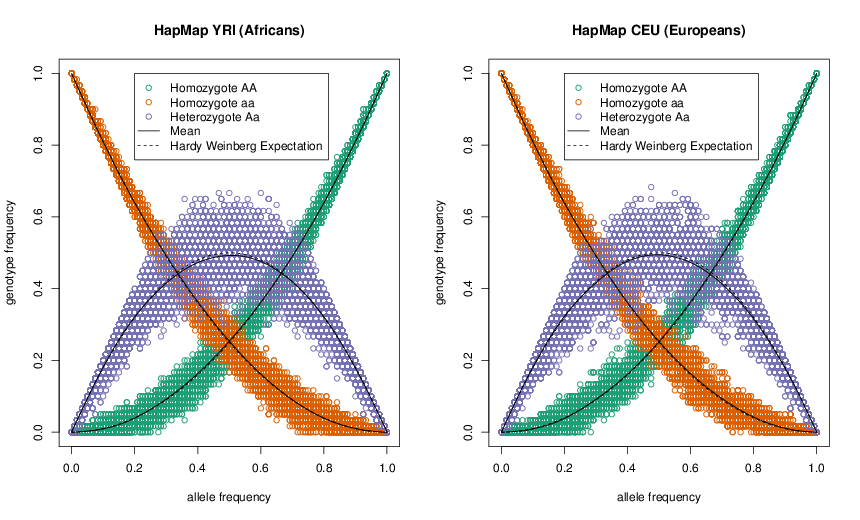
\includegraphics[width= \textwidth]{figures/CEU_YRI_separately_HWE.png}
\end{center}
\caption{Demonstrating Hardy--Weinberg proportions using 10,000 SNPs
  from the HapMap European (CEU)  and African (YRI) populations. Within
  each of these populations the allele frequency against the
  frequency of the 3 genotypes; each SNP is represented by 3 different
  coloured points. The solid lines show the mean genotype frequency. The dashed lines show the
  predicted genotype frequency from Hardy--Weinberg
  equilibrium. \gitcode{https://github.com/cooplab/popgen-notes/blob/master/Rcode/HWE_exercise/HWE_HAPMAP.R} Blog
  post on figure \href{http://gcbias.org/2011/10/13/population-genetics-course-resources-Hardy--Weinberg-eq/}{here}. } \label{fig:HWE_CEU_YRI}  %See \href{blog
                                %post}{http://gcbias.org/2011/10/13/population-genetics-course-resources-Hardy--Weinberg-eq/}
                                %here on this plot.  https://github.com/cooplab/popgen-notes/blob/master/Rcode/HWE_exercise/HWE_HAPMAP.R
\end{figure}

\begin{question}
You are investigating a locus with three alleles, A, B, and C, with
allele frequencies $p_A$, $p_B$, and $p_C$. What fraction of the
population is expected to be homozygotes under Hardy--Weinberg?
\end{question}

Microsatellites are regions of the genome where individuals vary for
the number of copies of some short DNA repeat that they carry. These
regions are often highly variable across individuals, making them
a suitable way to identify individuals from a DNA sample. This
so-called DNA fingerprinting has a range of applications from
establishing paternity and identifying human remains to matching
individuals to DNA samples from a crime scene. The FBI make use of the
CODIS database\sidenote{CODIS: Combined DNA Index System}. The CODIS
database contains the genotypes of over 13 million people, most of
whom have been convicted of a crime. Most of
the profiles record genotypes at 13 microsatellite loci that are
tetranucleotide repeats (since 2017, 20 sites have been genotyped).

The allele counts for two loci (D16S539
and TH01) are shown in table \ref{table:CODIS_1} and
\ref{table:CODIS_2} for a sample of 155 people of European ancestry. You can assume these two loci are on different chromosomes.

\begin{table}
{\small
\setlength{\tabcolsep}{.45\tabcolsep}
\csvautobooktabular{Rcode/CODIS/D16S539_counts.csv}  \label{table:CODIS_1}
\caption{ Data for 155 Europeans at the D16S539 microsatellite from
  CODIS from \citet{algee:16}. The top row gives the number of
  tetranucleotide repeats for each allele, the bottom row gives the
  sample counts.}
 }

\end{table}
\vspace*{1cm}
\begin{table}
  {\small
\setlength{\tabcolsep}{.45\tabcolsep}
\csvautobooktabular{Rcode/CODIS/TH01_counts.csv}  \label{table:CODIS_2}
}

\caption{Same as \ref{table:CODIS_1} but for the TH01 microsatellite. }
\end{table}

\begin{question} \label{Q:CODIS}
You extract a DNA sample from a crime scene. The genotype is 100/80 at the
D16S539 locus and 70/93 at TH01.\\

{\bf A)} You have a suspect in custody. Assuming this suspect is innocent and of European ancestry, what is the probability
that their genotype would match this profile by chance (a false-match probability)?\\
{\bf B)} The FBI uses $\geq 13$ markers. Why is this higher number
necessary to make the match statement convincing evidence in court?\\
{\bf C)}  An early case that triggered debate among forensic geneticists was a crime among the Abenaki, a Native American community in
Vermont \citep[see ][ for discussion]{lewontin:94}. There was a DNA sample from the crime scene, and the
perpetrator was thought likely to be a member of the Abenaki
community. Given that allele frequencies vary among populations, why would people be concerned about using data from a non-Abenaki population to compute a false match probability?
%---that is, the probability
%that a suspect's DNA would match a crime-scene sample if he were unrelated to anyone present at the crime scene
\end{question}

%\begin{question}
%Suppose the following genotype frequencies were observed for at an esterase locus in a population of Drosophila (A denotes the “fast” allele and B denotes the “slow” allele):
%\begin{center}
%\begin{tabular}{|ccc|}
%AA &	AB &	BB\\
%0.6 &	0.2 &	0.2\\
%\end{tabular}\,.
%\end{center}
%What genotype frequencies would you expect under Hardy Weinberg expectations?
%\end{question}


%%%ADD A comment about WF sampling here!
%% Also add a question about Poisson offspring number.

%\begin{figure}
%\begin{center}
%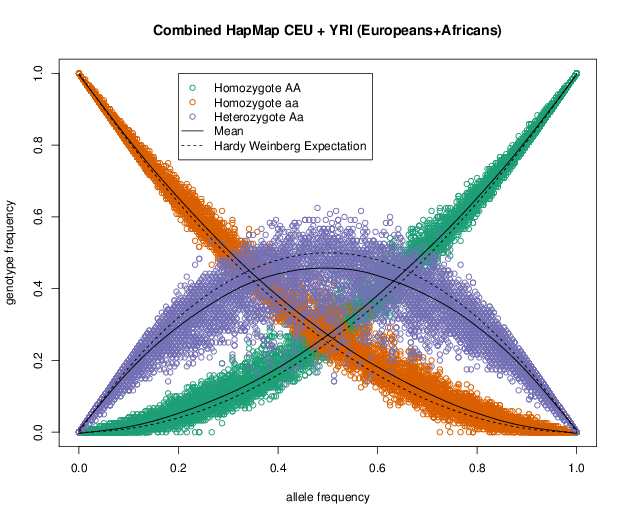
\includegraphics[width=0.5 \textwidth]{figures/CEU_YRI_together_HWE.png}
%\end{center}
%\caption{}
%\end{figure}


%figure/QT1.eps

\section{Allele sharing among related individuals and Identity by Descent}

All of the individuals in a population are related to each other by a giant
pedigree (family tree). For most pairs of individuals in a population these
relationships are very distant (e.g. distant cousins), while some individuals
will be more closely related (e.g. sibling/first cousins). All individuals
are related to one another by varying levels of relatedness, or \emph{kinship}.
Related individuals can share alleles that have both descended from the shared
common ancestor. To be shared, these alleles must be inherited through all
meioses connecting the two individuals (e.g. surviving the $\nicefrac{1}{2}$
probability of segregation each meiosis). As closer relatives are separated by
fewer meioses, closer relatives share more alleles. In Figure
\ref{fig:IBD_cousins_chr_cartoon} we show the sharing of chromosomal regions
between two cousins. As we'll see, many population and quantitative genetic
concepts rely on how closely related individuals are, and thus we need some way
to quantify the degree of kinship among individuals. \\
\begin{figure}
\begin{center}
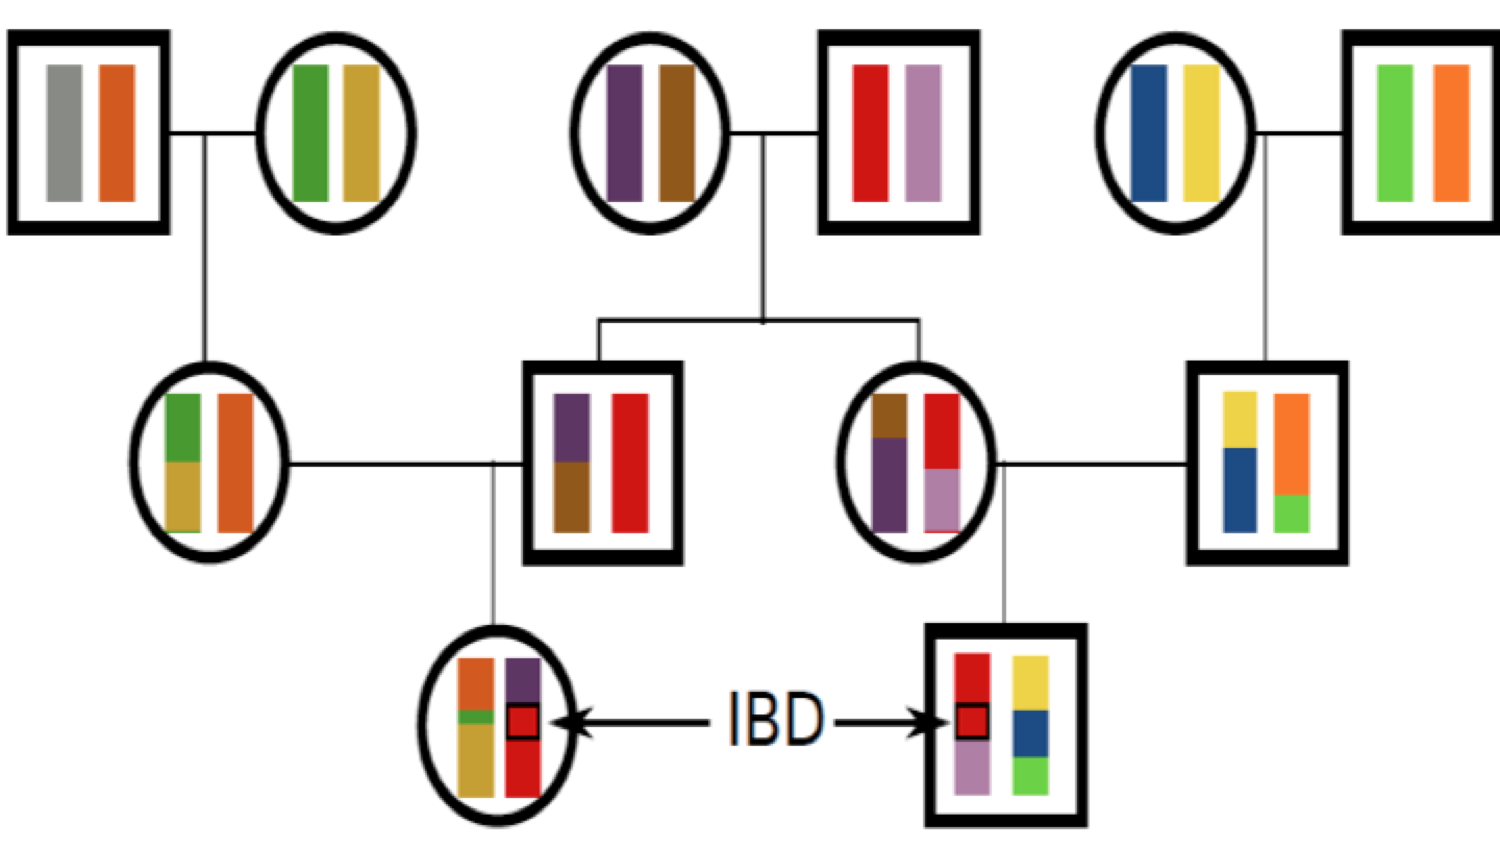
\includegraphics[width= 0.75 \textwidth]{figures/Cousins_IBD_chromo_cartoon.png}
\end{center}
\caption{First cousins sharing a stretch of chromosome identical by
  descent. The different grandparental diploid chromosomes are coloured so we
  can track them and recombinations between them across the
  generations. Notice that the identity by descent between the cousins persists for a long
stretch of chromosome due to the limited number of generations for
recombination. The squares represent males and circles females. } \label{fig:IBD_cousins_chr_cartoon}
\end{figure}

We will define two alleles to be identical by descent (IBD) if they are
identical due to transmission from a common ancestor in the past few generations\cite{cotterman:40,malecot:48}. For the moment,
we ignore mutation, and we will be more precise about what we mean by `past few
generations' later on. For example, parent and child share exactly one allele
identical by descent at a locus, assuming that the two parents of the child are
randomly mated individuals from the population. In Figure
\ref{fig:IBD_cousins_cartoon}, I show a pedigree demonstrating some
configurations of IBD. \\

\marginnote{Here we'll focus on IBD of outbred individuals. Dealing
  with sharing between inbred individuals requires $6$ more  identity-by-descent
$r$ coefficients, which honestly makes my head spin.}
One summary of how related two individuals are is the probability that our pair
of individuals share 0, 1, or 2 alleles identical by descent (see Figure
\ref{fig:IBD_0_1_2}). We denote these  identity-by-descent probabilities by $r_0$, $r_1$, and $r_2$
respectively. See Table \ref{table:IBDprobs} for some examples. We can also
interpret these probabilities as genome-wide averages. For example, on average, at a quarter of all their autosomal loci
full-sibs share zero alleles identical by descent.\\



One summary of relatedness that will be important is the probability that two
alleles ($I$ \& $J$) picked at random, one from each of the two different individuals $i$
and $j$, are identical by descent ($P(\text{I\&J IBD})$). We call this quantity the \emph{coefficient
of kinship} of individuals $i$ and $j$, and denote it by $F_{ij}$. It is
calculated as
%JRI: you come back to inbreeding later, but perhaps worth mentioning here that you are only considering outbred Individuals

\begin{align}
  F_{ij} = & P(\text{I\&J IBD} )\\
  =& P(\text{I\&J IBD} |~ \text{i\&j  0 IBD}) P(\text{i\&j  0 IBD})  \nonumber\\
  & + P(\text{I\&J IBD} |~ \text{i\&j  1 IBD})
    P(\text{i\&j  1 IBD})  \nonumber\\
  &+ P(\text{I\&J IBD} |~ \text{i\&j  2 IBD}) P(\text{i\&j  2 IBD}) \label{eqn:coeffkinship_step}\\
   =   &   0 \times r_0 + \frac{1}{4} r_1  + \frac{1}{2} r_2.
\label{eqn:coeffkinship}
\end{align}
\begin{marginfigure}[-1cm]
\begin{center}
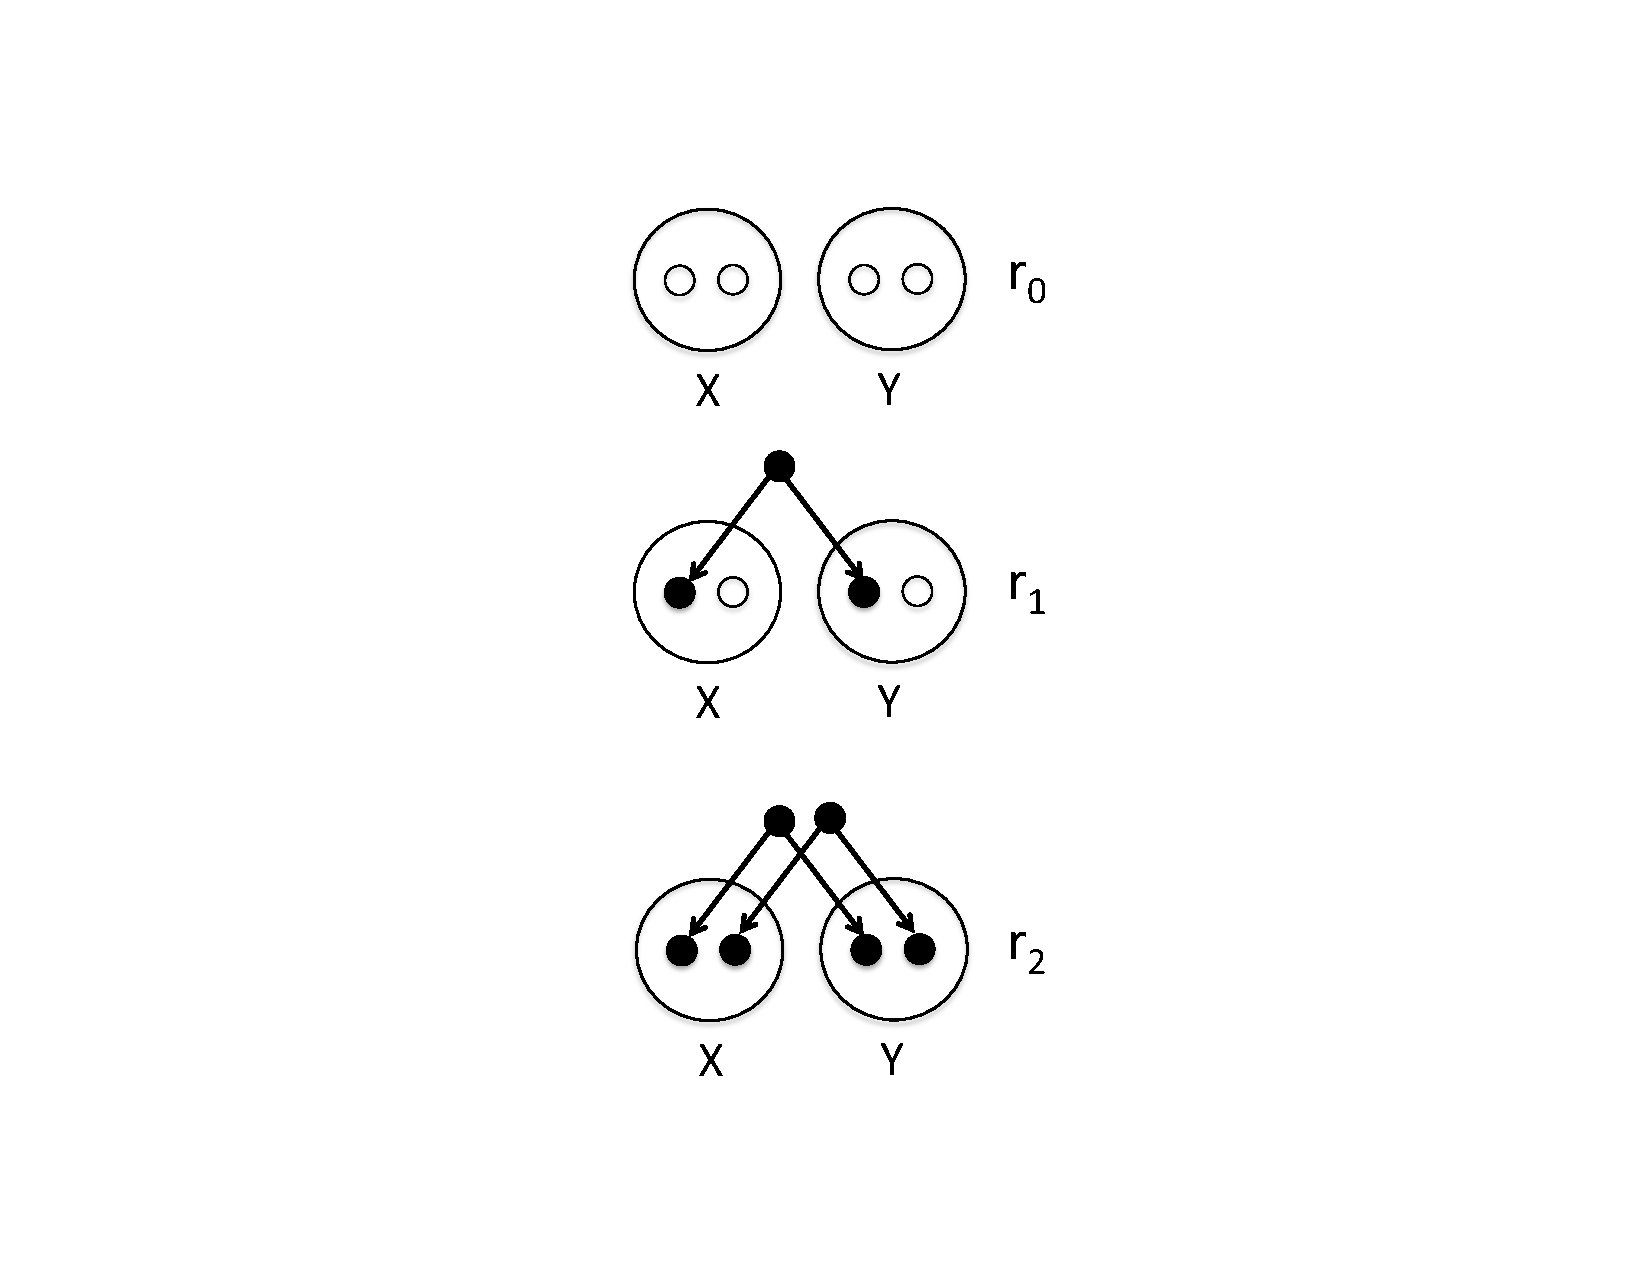
\includegraphics[width= 0.75 \textwidth]{figures/sharing_relatives/IBD_0_1_2.pdf}
\end{center}
\caption{A pair of diploid individuals (i and j) sharing 0, 1, or 2 alleles IBD
  where lines show the sharing of alleles by descent (e.g. from a
  shared ancestor). } \label{fig:IBD_0_1_2}
\end{marginfigure}

In the above step, eqn\eqref{eqn:coeffkinship_step}, we're summing the
conditional probability of alleles $I$ \& $J$ being IBD over whether our individuals $i$ \& $j$ share $0$, $1$,
or $2$ alleles IBD, an example of using the Law of Total Probability (see Appendix
eqn \eqref{eqn:law_tot_prob}).  We've then, in eqn \ref{eqn:coeffkinship}, used the fact that we can
calculate our condition probabilities of  I \& J being IBD using the
rules of Mendelian transmision. Consider the probability $
P(\text{I\&J IBD} |~ \text{i\&j  1 IBD})$, i.e. that our
pair of alleles ($I$ \& $J$) drawn from individuals $i$ and $j$ are IBD given that
$i$ and $j$ share one allele IBD, this is a $\nicefrac{1}{4}$ as we need to
draw the allele that is IBD from both $i$ and $j$, i.e. drawing both black
alleles in the middle panel of Figure \ref{fig:IBD_0_1_2}, which
happens with probability $\nicefrac{1}{2} \times \nicefrac{1}{2} $. 
The coefficient of kinship will appear multiple times, in both our discussion of
inbreeding and in the context of phenotypic resemblance between relatives.\\

\begin{table*}
\begin{center}
\begin{tabular}{ l c c c c}
\hline
Relationship (i,j)$^{*}$ & $P(\text{i\&j  0 IBD}) $ & $P(\text{i\&j  1 IBD}) $ & $P(\text{i\&j  2 IBD}) $ & $P(\text{I\&J IBD} )$\\
  \hline
  Relationship (i,j)$^{*}$ & $r_0$ & $r_1$ & $r_2$ & $F_{ij}$\\
    \hline
parent--child & 0 & 1 & 0 & \nicefrac{1}{4}\\
full siblings & \nicefrac{1}{4} & \nicefrac{1}{2} & \nicefrac{1}{4} & \nicefrac{1}{4}\\
Monozygotic twins  & 0 & 0 & 1  & \nicefrac{1}{2} \\
$1^{st}$ cousins & \nicefrac{3}{4} & \nicefrac{1}{4} & 0 & \nicefrac{1}{16}\\
\hline
\end{tabular}
\end{center}
\caption{Probability that two individuals of a given relationship share 0, 1, or 2 alleles
identical by descent on the autosomes. $^{*}$Assuming that our
individuals are outbred and that this the only close relationship the pair shares. } % doesn't this implicitly assume an infinite population?
\label{table:IBDprobs}
\end{table*}

\begin{question}
  What are $r_0$, $r_1$, and $r_2$ for $\nicefrac{1}{2}$ sibs? ($\nicefrac{1}{2}$ sibs share one
parent but not the other).
\end{question}

\begin{question}
  Explain in words why $ P(\text{I\&J IBD} |~ \text{i\&j  2 IBD}) = \nicefrac{1}{2}$.
\end{question}

%Question 5. Consider a biallelic locus where allele 1 is at fre- quency p, and two individuals who have IBD allele sharing probabili- ties r0, r1, r2.
%What is the overall probability that these two individuals are both homozygous for allele 1?

\paragraph{Genotypic sharing between pairs of individuals.}
Our $r$ coefficients are going to have various uses. For example, they allow us
to calculate the probability of the genotypes of a pair of
relatives. Consider a biallelic locus where allele $A_1$ is
at frequency $p$, and two individuals who have IBD allele sharing
probabilities $r_0$, $r_1$, $r_2$. What is the overall probability that these
two individuals are both homozygous for allele 1? Well that's
\begin{align}
  P(A_1 A_1) = & P(A_1 A_1 | \text{0 alleles IBD}) P(\text{0 alleles IBD})  \nonumber\\
  & + P(A_1 A_1 | \text{1 allele IBD}) P(\text{1 allele IBD})  \nonumber\\
  &+ P(A_1 A_1 | \text{2 alleles IBD}) P(\text{2 alleles IBD})
\end{align}
Or, in our $r_0$, $r_1$, $r_2$ notation:
\begin{align}
  P(A_1 A_1) = & P(A_1 A_1 | \text{0 alleles IBD}) r_0  \nonumber\\
  & + P(A_1 A_1 |
  \text{1 alleles IBD}) r_1  \nonumber\\
  & + P(A_1 A_1 | \text{2 alleles IBD}) r_2 \label{eqn:initial_relly_IBD_calc}
\end{align}
If our pair of relatives share $0$ alleles IBD, then the probability that
they are both homozygous is $P(A_1 A_1 |
\text{0 alleles IBD}) =p^2 \times p^2$, as all four alleles
represent independent draws from the population. If they share $1$
allele IBD, then the shared allele is of type $A_1$ with probability $p$, and then
the other non-IBD allele, in both relatives, also needs
to be $A_1$ which happens with probability $p^2$, so $P(A_1 A_1 |
\text{1 alleles IBD})=p \times p^2$. Finally, our pair of relatives can
share two alleles IBD, in which case $P(A_1 A_1 | \text{2 alleles IBD})
= p^2$, because if one of our individuals is homozygous for the $A_1$ allele,
both individuals will be. Putting this all together our equation
\eqref{eqn:initial_relly_IBD_calc} becomes
\begin{equation}
P(A_1 A_1) = p^4 r_0 + p^3 r_1 + p^2 r_2 \label{eqn:IBD_relly_calc}
\end{equation}
Note that for specific cases we could also calculate this by summing over all the
possible genotypes their shared ancestor(s) had; however, that would be much more
involved and not as general as the form we have derived here.

We can write out terms like eq \eqref{eqn:IBD_relly_calc} for all of
the possible configurations of genotype
sharing/non-sharing between a pair of individuals. Based on this we can write down the expected number of
polymorphic sites where our individuals are observed to share 0, 1, or 2
alleles.

\begin{question} [Trickier question.]
The genotype of our suspect in Question \ref{Q:CODIS} turns out to be 100/80 for
D16S539 and 70/80 at TH01. The suspect is not a match to the DNA
from the crime scene; however, they could be a sibling.

Calculate the joint probability of observing the genotype from the crime and our
suspect:\\
{\bf A)} Assuming that they share no close relationship.\\
%JRI: pretty sure the answer key is wrong here. If we put your eact set of fractions into R we get 1.433992e-09 as the answer. So something is wrong somewhere in answer.

{\bf B)} Assuming that they are full sibs.\\

{\bf C)} Briefly explain your findings.
  \end{question}

 \begin{marginfigure}
\begin{center}
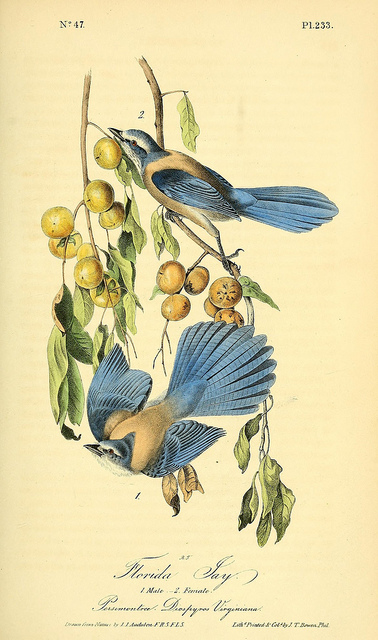
\includegraphics[width= \textwidth]{illustration_images/alleles_genotypes/Florida_scrub_jay/8576533889_3a131ffc4c_z.jpg}
\end{center}
\caption{Florida Scrub-Jays ({\it Aphelocoma coerulescens}). \BHLCC{The birds of America : from drawings made in the United
    States and their territories. 1880. Audubon
    J.J.}{https://www.biodiversitylibrary.org/page/40447048\#page/169/mode/1up}{Smithsonian
    Libraries}{2.0} } \label{fig:FSJ}
\end{marginfigure}


There's a variety of ways to estimate the relationships among
individuals using genetic data.  An example of using allele sharing to identify relatives is offered by
the work of Nancy Chen \citep[in collaboration with Stepfanie
Aguillon, see ][]{chen:16,Aguillon:17}. \citeauthor{chen:16} has collected genotyping data from thousands of
Florida Scrub Jays at over ten thousand loci. These Jays live at the
Archbold field site, and have been carefully monitored for many
decades allowing the pedigree of many of the birds to be known.
Using these data she estimates allele frequencies at each
locus. Then by equating the observed number of times that a pair of
individuals share $0$, $1$, or $2$ alleles to the theoretical
expectation, she estimates the probability of $r_0$, $r_1$, and
$r_2$ for each pair of birds. A plot of these are shown in Figure
\ref{fig:FSJ_IBD}, showing how well the estimates match those known
from the pedigree.
%\end{question}


\begin{figure}
\begin{center}
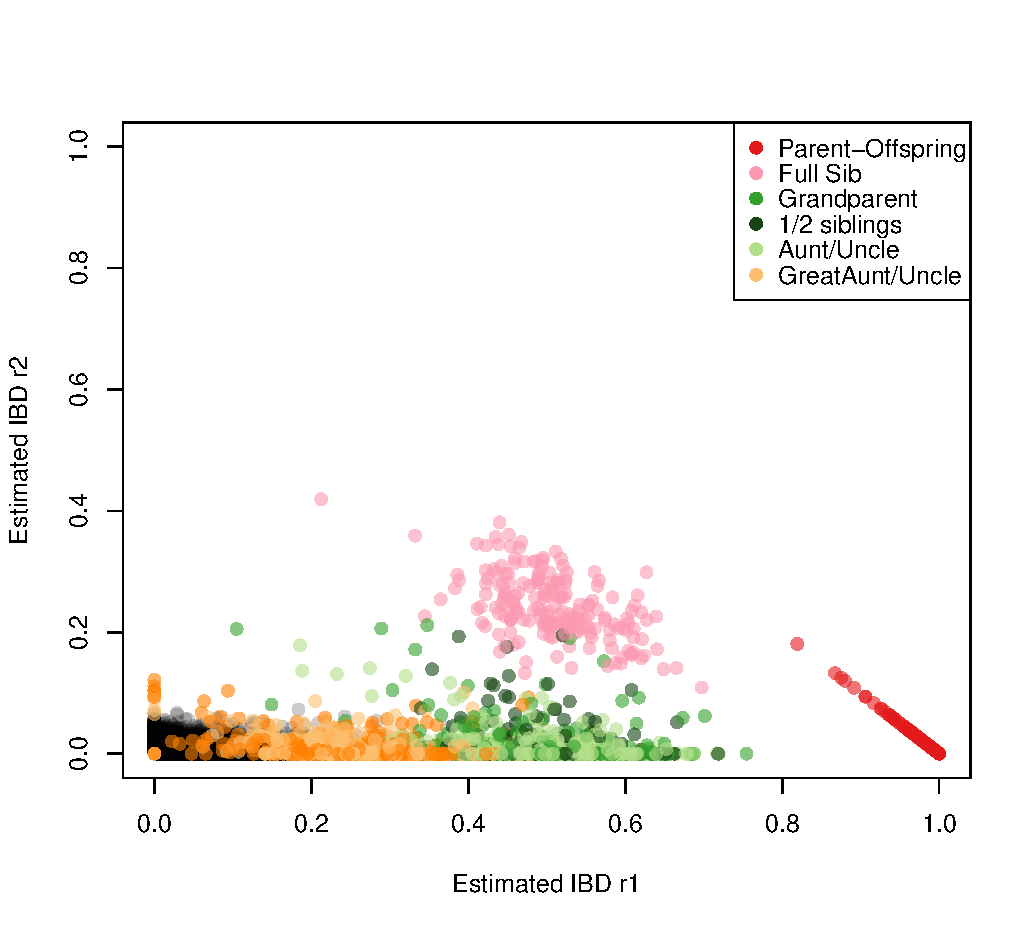
\includegraphics[width= 0.75 \textwidth]{figures/FSJ_IBD.pdf}
\end{center}
\caption[3cm]{Estimated coefficient
of kinship from Florida Scrub Jays. Each point is a pair of
individuals, plotted by their estimated IBD ($r_1$ and $r_2$) from their genetic data. The
points are coloured by their known pedigree relationships. Note that
most pairs have low kinship, and no recent genealogical relationship,
and so appear as black points in the lower left corner. Thanks to
Nancy Chen for supplying the data. \gitcode{https://github.com/cooplab/popgen-notes/blob/master/Rcode/FSJ_IBD/FSJ_IBD_plotting.R} } \label{fig:FSJ_IBD}
\end{figure}

\paragraph{Sharing of genomic blocks among relatives.}
\begin{figure}
\begin{center}
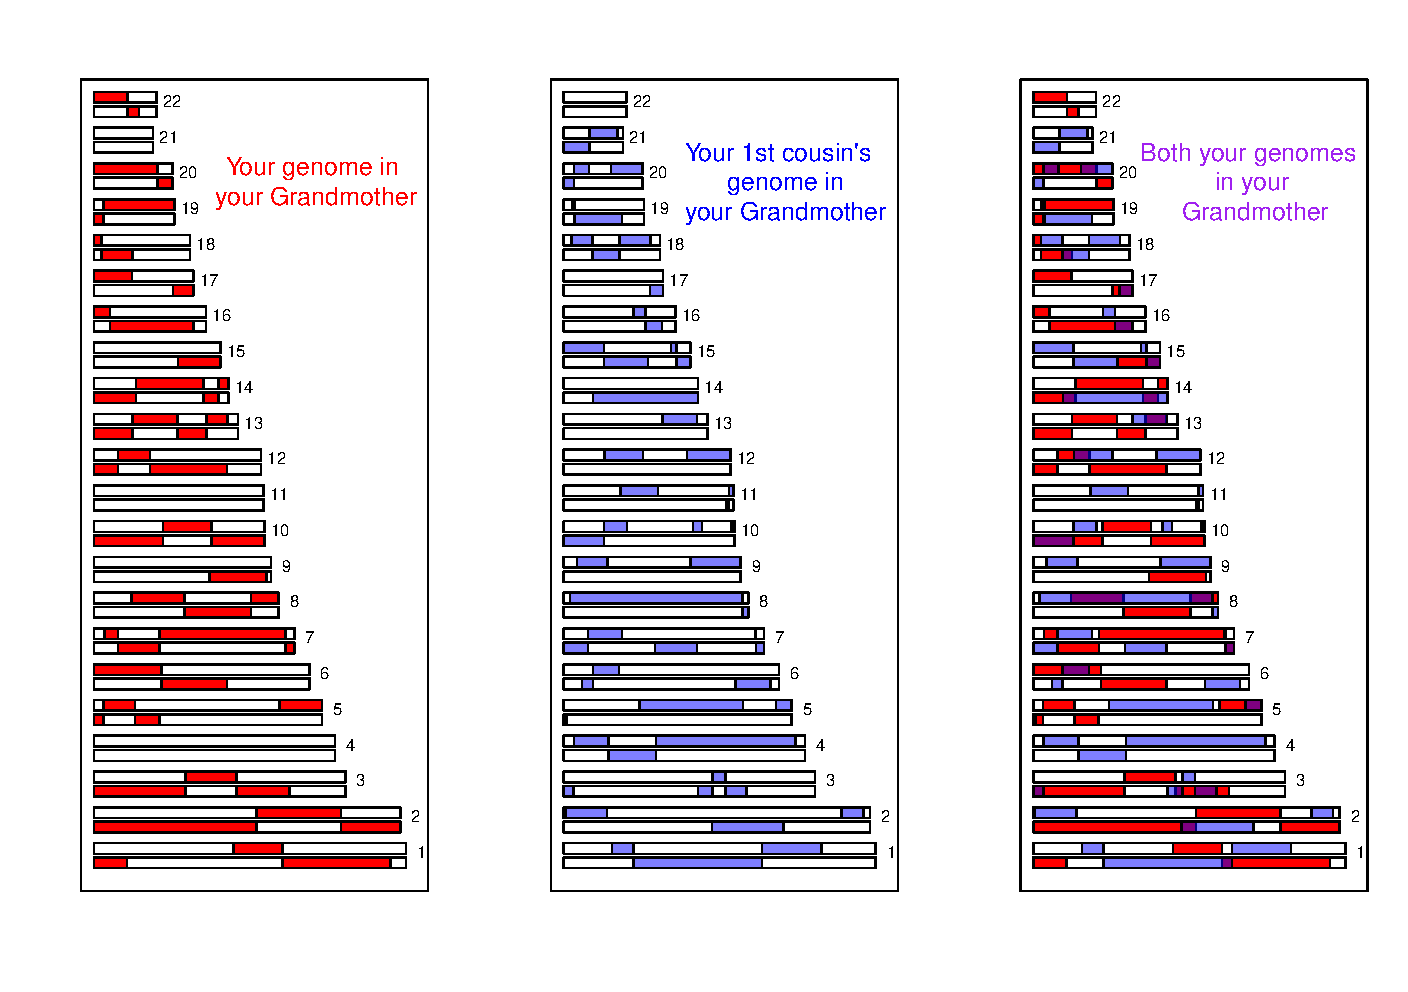
\includegraphics[width= \textwidth]{figures/sharing_relatives/First_cousin_overlap.pdf}
\end{center}
\caption[]{A simulation of sharing between first cousins. The regions of your grandmother's 22 autosomes that you inherited are
coloured red, those that your cousins inherited are coloured blue. In the third panel we show the overlapping genomic regions in purple, these regions will be IBD in you and your cousin. If you are full first cousins, you will also have shared genomic regions from your shared grandfather, not shown here. Details about how we made these simulations \href{https://gcbias.org/2013/12/02/how-many-genomic-blocks-do-you-share-with-a-cousin/}{here}.
} \label{fig:first_cousin_IBD}
\end{figure}
We can more directly see the sharing of the genome among close
relatives using high-density SNP genotyping arrays. In Figure \ref{fig:first_cousin_IBD} we show a simulation of you and your first cousin's genomic material that you both inherited from your shared grandmother. Colored purple are regions where you and your cousin will have matching genomic material, due to having inherited it IBD from your shared grandmother.
%JRI: text says ``Below'' but float ends up above



You and your first cousin will share at least one allele of your genotype at all of the polymorphic loci in these purple regions. There's a range of methods to detect such sharing. One way is to look for unusually long stretches of the genome where two individuals are never homozygous for different alleles. By identifying pairs of individuals who share an unusually large number of such putative IBD blocks, we can hope to identify unknown relatives in genotyping datasets. In fact, companies like 23\&me and Ancestry.com use signals of IBD to help identify family ties.

As another example, consider the case of third cousins. You share one of eight sets of great-great grandparents with each of your (likely many) third cousins. On average, you and each of your third cousins each inherit one-sixteenth of your genome from each of those two great-great grandparents. This turns out to imply that on average, a little less than one percent of your and your third cousin's genomes ($2 \times (1/16)^2 =0.78\%$) will be identical by virtue of descent from those shared ancestors. A simulated example where third cousins share blocks of their genome (on chromosome 16 and 2) due to their great, great grandmother is shown in Figure \ref{fig:third_cousin_IBD}.

\begin{figure}
\begin{center}
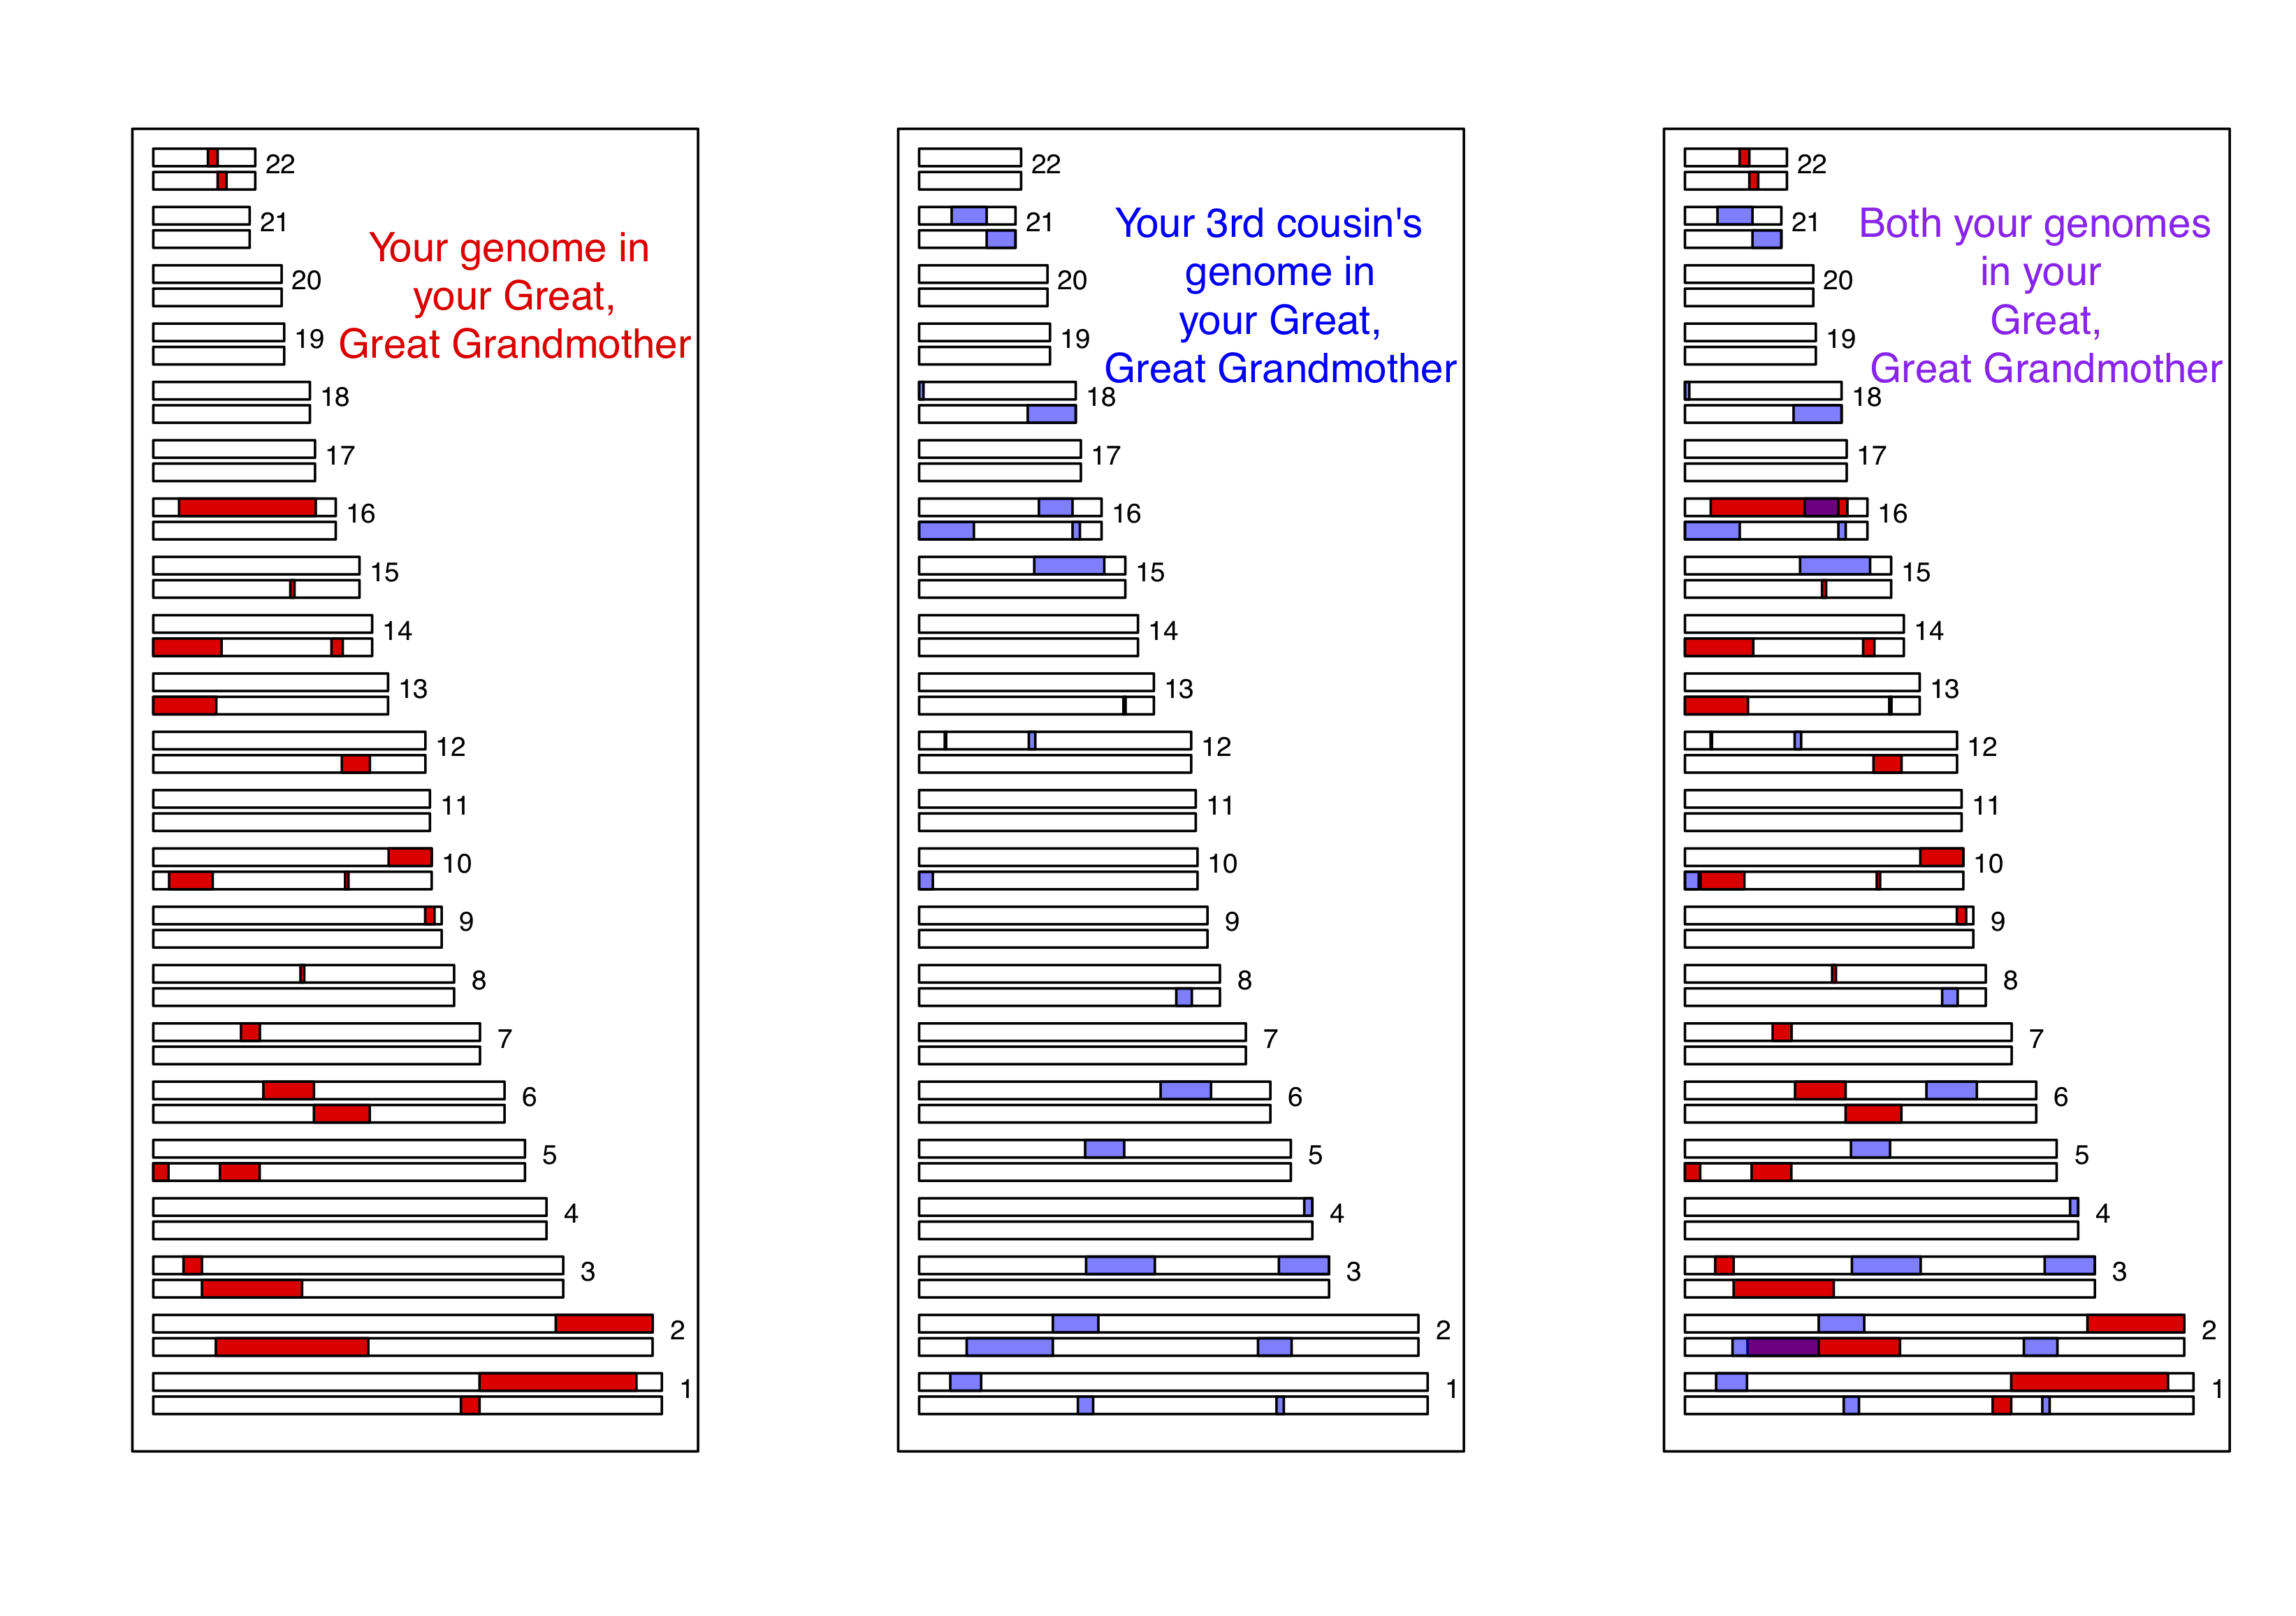
\includegraphics[width= \textwidth]{figures/sharing_relatives/Third_cousin_overlap_1.png}
\end{center}
\caption[]{A simulation of sharing between third cousins, the details are the same as in Figure \ref{fig:first_cousin_IBD}.} \label{fig:third_cousin_IBD}
\end{figure}


Note how if you compare Figure \ref{fig:third_cousin_IBD} and Figure \ref{fig:first_cousin_IBD}, individuals inherit less IBD from a shared great, great grandmother than from a shared grandmother, as they inherit from more total ancestors further back. Also notice how the sharing occurs in shorter genomic blocks, as it has passed through more generations of recombination during meiosis. These blocks are still detectable, and so third cousins can be detected using high-density genotyping chips, allowing more distant relatives to be identified than single marker methods alone. \sidenote{Indeed the suspect in case of the Golden State Killer was identified through identifying third cousins that genetically matched a DNA sample from an old crime scene (see \href{https://gcbias.org/2018/05/07/how-lucky-was-the-genetic-investigation-in-the-golden-state-killer-case/}{here} for more details).} More distant relations than third cousins, e.g. fourth cousins, start to have a significant probability of sharing none of their genome IBD. But you have many fourth cousins, so you will share some of your genome IBD with some of them; however, it gets increasingly hard to identify the degree of relatedness from genetic data the deeper in the family tree this sharing goes.

\subsection{Inbreeding}
We can define an inbred individual as an individual whose parents are
more closely related to each other than two random individuals drawn
from some reference population.  \\


\begin{marginfigure}
\begin{center}
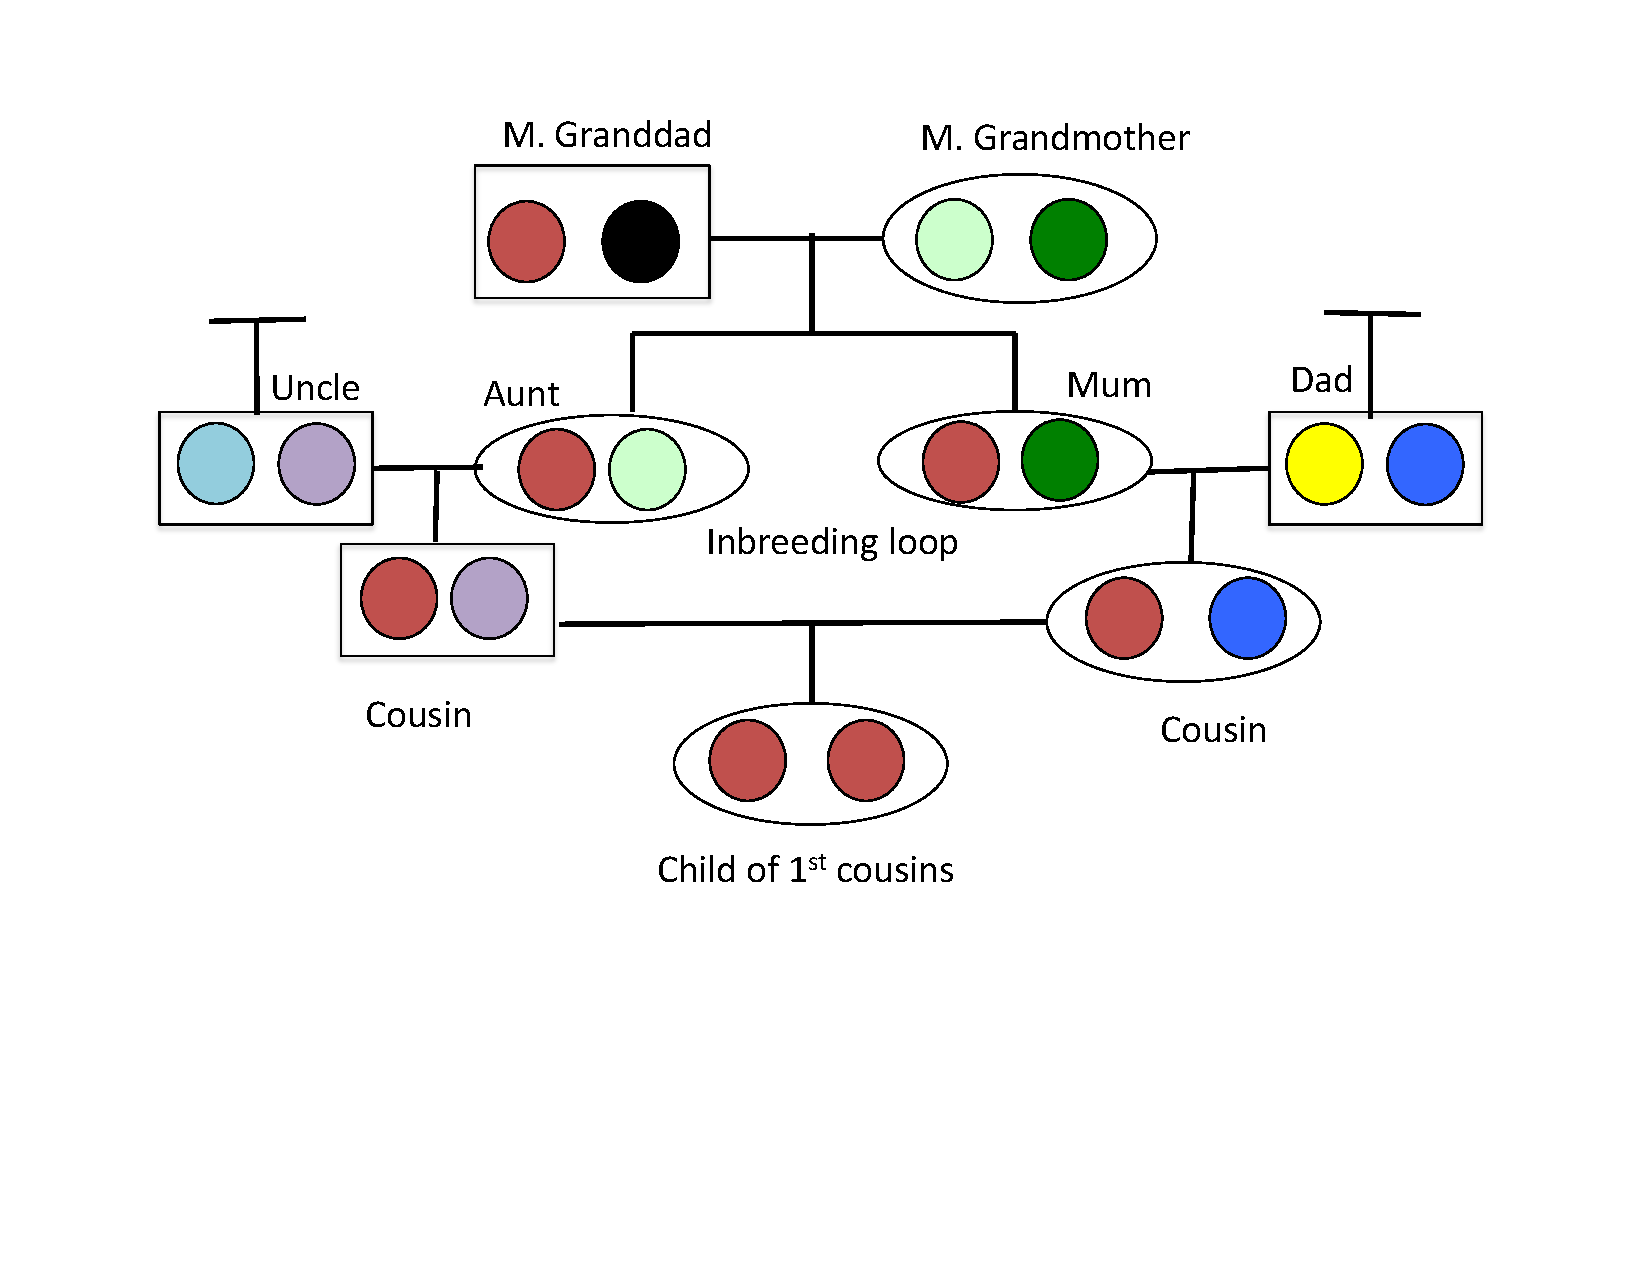
\includegraphics[width= \textwidth]{figures/Child_first_cousins_Homozy_BD.pdf}
\end{center}
\caption{Alleles being transmitted through an inbred pedigree. The two sisters (mum and aunt) share two alleles identical by descent (IBD). The cousins share one
  allele IBD. The offspring of first cousins is homozygous by
  descent at this locus.} \label{fig:IBD_cousins_cartoon}
\end{marginfigure}
\graham{Change this to have squares and circles}
When two related individuals produce an offspring, that individual can
receive two alleles that are identical by descent, i.e.\ they
can be homozygous by descent (sometimes termed autozygous), due to the
fact that they have two copies of an allele through different paths
through the pedigree.  This increased likelihood of being homozygous
relative to an outbred individual is the most obvious effect of
inbreeding. It is also the one that will be of most interest to us, as it
underlies a lot of our ideas about inbreeding depression and
population structure. For example, in Figure \ref{fig:IBD_cousins_cartoon} our
offspring of first cousins is homozygous by descent having received
the same IBD allele via two different routes around an inbreeding loop.\\

As the offspring receives a random allele from each parent ($i$ and $j$), the
probability that those two alleles are identical by descent is equal to the
kinship coefficient $F_{ij}$ of the two parents (Eqn.\ \ref{eqn:coeffkinship}). This follows from the fact that
the genotype of the offspring is made by sampling an allele at random from each
of our parents. % We will use IBD for identical by descent. \\ %% this was already defined above.

\begin{table}
\begin{center}
\begin{tabular}{ccc}
\hline
$f_{11}$ & $f_{12}$ & $f_{22}$ \\
\hline
$(1-F) p^2 + F p$ & $(1-F) 2pq$ & $(1-F) q^2 + F q$ \\
\hline
\end{tabular}
\end{center}
\caption{\textbf{Generalized Hardy--Weinberg}} \label{table:GeneralizedHWE}
\end{table}

The only way the offspring can be heterozygous ($A_1 A_2$) is if their two
alleles at a locus are not IBD (otherwise they would necessarily be
homozygous). Therefore, the probability that they are heterozygous is

\begin{equation}
(1-F) 2p q,
\label{eq:hetGenHW}
\end{equation}
%
where we have dropped the indices $i$ and $j$ for simplicity.  The offspring
can be homozygous for the $A_1$ allele in two different ways.  They can have
two non-IBD alleles that are not IBD but happen to be of the allelic type
$A_1$, or their two alleles can be IBD, such that they inherited allele $A_1$
by two different routes from the same ancestor. Thus, the probability that an
offspring is homozygous for $A_1$ is

\begin{equation}
(1-F) p^2 + F p.
\end{equation}
%
Therefore, the frequencies of the three possible genotypes can be written as given in
Table \ref{table:GeneralizedHWE}, which provides a generalization of the Hardy--Weinberg
proportions.\\


%Note that the generalized Hardy--Weinberg proportions completely
%specify the genotype probabilities, as there are two parameters ($p$ and $F$)
%and two degrees of freedom (as $p$ and $q$ have to sum to one).
%Therefore, any combination of genotype frequencies at a biallelic site
%can be specified by a combination of $p$ and $F$.\\
%JRI: unclear to me if this is useful. will readers understand parameter numbers/DF?

\begin{question}
The frequency of the $A_1$ allele is $p$ at a biallelic locus. Assume that our population is randomly mating and that the
genotype frequencies in the population follow from HW. We select two
individuals at random to mate from this population. We then mate the children
from this cross. What is the probability that the child from this full
sib-mating is
homozygous?
\end{question}

\paragraph{Multiple inbreeding loops in a pedigree.}
Up to this point we have assumed that there is at most one inbreeding loop in the recent family history of our
  individuals, i.e. the parents of our inbred individual have at most one recent genealogical connection. However, an individual who has multiple inbreeding loops in their pedigree can be homozygous by
  descent thanks to receiving IBD alleles via multiple different different loops. To calculate inbreeding in pedigrees of arbitrary complexity, we can extend
 beyond our original relatedness coefficients $r_0$, $r_1$, and $r_2$ to account for
 higher order sharing of alleles IBD among relatives. For example,
 we can ask, what is the probability that \textit{both} of the alleles in the first individual
 are shared IBD with one allele in the second individual? There are
 nine possible relatedness coefficients in total to completely describe kinship between two diploid individuals, and we won't go in to them here
 as it's a lot to keep track of.
However, we will show how we can calculate the inbreeding coefficient of an
individual with multiple inbreeding loops more directly.\\

%ut at loci where the ancestor is inbred you get two more options (C inherits maternal/B paternal or opp.) so the factor of 2 applies to fA as well and cancels out for both.}

Let's say the parents of our inbred individual (B and C) have $K$ shared ancestors,
i.e. individuals who appear in both B and C's recent family trees. We denote these shared ancestors by $A_1, \dots,A_K$, and we denote by $n$ the total number of individuals in the chain from B to C via ancestor $A_i$, including B, C, and $A_i$. For example, if B is C's aunt, then B and C share two ancestors, which are B's parents and, equivalently, C's grandparents. In this case, there are n=4 individuals from B to C through each of these two shared ancestor. In the general case, the kinship coefficient of B and C,
i.e. the inbreeding coefficient of their child, is
\begin{equation}
 F = \sum_{i=1}^K \frac{1}{2^{n_i}} \big( 1+ f_{A_i} \big)
\end{equation}
where $f_{A_i}$ is the inbreeding coefficient of the ancestor
$A_i$. What's happening here is that we sum over all the mutually-exclusive paths in the pedigree through which B and C can share an allele IBD. With probability
$\nicefrac{1}{2^{n_i}}$, a pair of alleles picked at random from B and C is descended from the same ancestral allele in individual
$A_i$, in which case the alleles are IBD. \sidenote{For example, in the case of our aunt-nephew case, assuming that the aunt's two parents are their only recent shared ancestors, then $F = \nicefrac{1}{2^4}+\nicefrac{1}{2^4} = \nicefrac{1}{8}$, in agreement with the answer we would obtain from  eqn \eqref{eqn:coeffkinship}.} However, even if B inherits the maternal allele and C inherits the paternal allele of shared ancestor $A_i$, if $A_i$ was
themselves inbred,  with probability $f_{A_i}$ those two
alleles are themselves IBD. Thus a shared \textit{inbred} ancestor further increases
the kinship of B and C.

\begin{figure}
  \begin{center}
  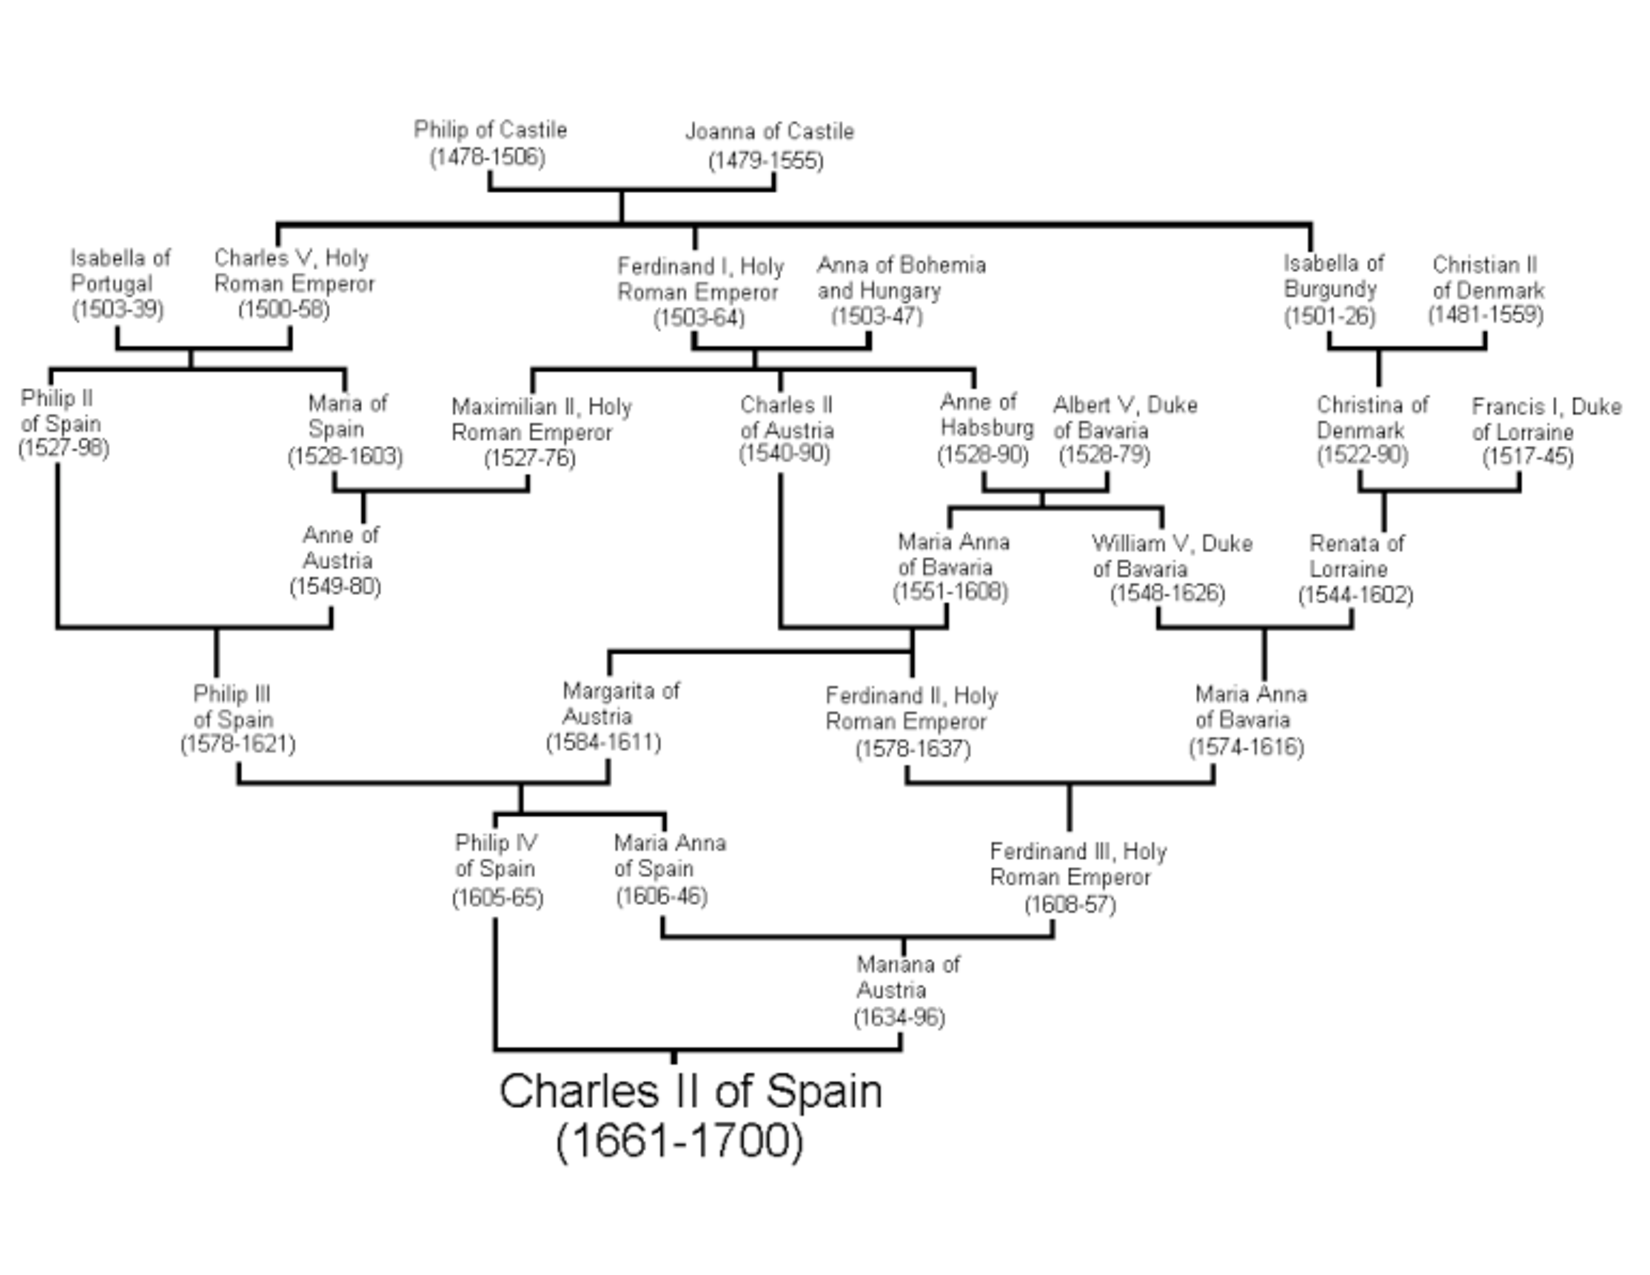
\includegraphics[width=
  \textwidth]{Journal_figs/alleles_genotypes/Charles_second_pedigree/Carlos_second_pedigree_2_trimmed.pdf}  %https://commons.wikimedia.org/wiki/File:Carlos_segundo80.png
\end{center}
\caption{The pedigree of King Charles II of
  Spain. Pedigree from
  \href{https://commons.wikimedia.org/wiki/File:Carlos_segundo80.png}{wikimedia}
drawn by \href{https://en.wikipedia.org/wiki/User:Lec_CRP1}{Lec CRP1},
public domain.} \label{fig:Carlos_second_pedigree}
\end{figure}
\begin{marginfigure}
\begin{center}
  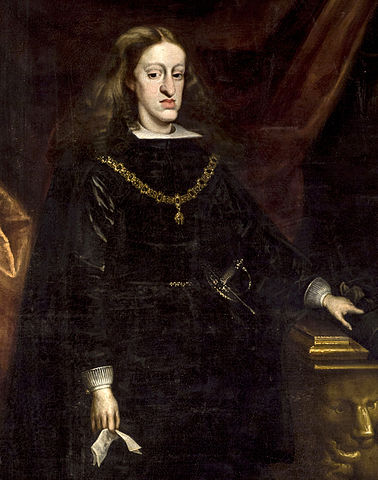
\includegraphics[width=
  \textwidth]{illustration_images/alleles_genotypes/Carlos_second/378px-Juan_de_Miranda_Carreno_002.jpg}
%https://commons.wikimedia.org/wiki/File:Carlos_segundo80.png
\end{center}
\caption{Charles II of Spain (by Juan Carre\~{n}o de Miranda,
  1685). \href{https://it.wikipedia.org/wiki/Carlo_II_di_Spagna\#/media/File:Juan_de_Miranda_Carreno_002.jpg}{Public Domain}.} \label{fig:Carlos_second}
\end{marginfigure}
Multiple inbreeding loops increase the probability that a child
is homozygous by descent at a locus, which can be calculated simply by plugging in $F$, the child's
inbreeding coefficient, into our generalized HW equation.


As one extreme example of the impact of multiple inbreeding loops in
an individual's pedigree, let's consider king Charles II of
Spain, the last of the Spanish Habsburgs.  Charles was the son of
Philip IV of Spain and Mariana of Austria, who were uncle and
niece. If this were the only inbreeding loop, then Charles would have had an
inbreeding coefficient of $\nicefrac{1}{8}$. Unfortunately for Charles, the
Spanish Habsburgs had long kept wealth and power within their family
by arranging marriages between close kin. The pedigree of Charles II is shown in Figure \ref{fig:Carlos_second_pedigree}, and
multiple inbreeding loops are apparent. For example, Phillip III,
Charles II's grandfather and great-grandfather, was himself a child of
an uncle-niece marriage.

\citet{alvarez:09} calculated that Charles II had an inbreeding
coefficient of $0.254$, equivalent to a full-sib mating,
thanks to all of the inbreeding loops in his pedigree. Therefore, he
is expected to have been homozygous by descent for a full quarter of his
genome. As we'll talk about later in these notes, this means that Charles
may have been homozygous for a number of recessive disease alleles,
and indeed he was a very sickly man who left no descendants due to his
infertility. \sidenote[][-2cm]{Pedro Gargantilla, who performed Charles's autopsy, stated
  that his body ``did not contain a single drop of blood; his heart was
  the size of a peppercorn; his lungs corroded; his intestines rotten
  and gangrenous; he had a single testicle, black as coal, and his
  head was full of water.'' While some of this description
  may refer to actual medical conditions, some of these details seem a
  little unlikely. See
  \href{https://www.thevintagenews.com/2017/03/23/when-charles-ii-of-spain-died-the-autopsy-stated-that-his-body-did-not-contain-a-single-drop-of-blood-and-his-head-was-full-of-water/}{here}.
} Thus plausibly the end of one of the great
European dynasties came about through inbreeding. 
%JRI: good idea to include links to potentially impermanent websites?


\subsection{Calculating inbreeding coefficients from genetic data}

%JRI: you transition from an individual's inbreeding coefficient here to using F as a population inbreeding parameter. i think some text explaining this change of scope might help

If the observed heterozygosity in a population is $H_O$, and we assume that the
generalized Hardy--Weinberg proportions hold, we can set $H_O$ equal to
$f_{12}$, and solve Eq.\ \eqref{eq:hetGenHW} for $F$ to obtain an estimate of
the inbreeding coefficient as

\begin{equation}
\hat{F} = 1-\frac{f_{12}}{2pq} = \frac{2pq - f_{12}}{2pq}.
\label{eqn:Fhat}
\end{equation}

As before, $p$ is the frequency of allele $A_{1}$ in the population. This can
be rewritten in terms of the observed heterozygosity ($H_O$) and the
heterozygosity expected in the absence of inbreeding, $H_E=2pq$, as
\begin{equation}
\hat{F} = \frac{H_E-H_O}{H_E} = 1 - \frac{H_O}{H_E}.
\label{eqn:FhatHO}
\end{equation}
Hence, $\hat{F}$ quantifies the deviation due to inbreeding of the observed heterozygosity from the one expected under random mating, relative to the latter.

\begin{question}
  Suppose the following genotype frequencies were observed for an esterase locus in a population of \textit{Drosophila} (A denotes the ``fast" allele and B denotes the ``slow" allele):
\begin{center}
\begin{tabular}{ccc}
\hline
AA &	AB &	BB\\
\hline
0.6 &	0.2 &	0.2\\
\end{tabular}
\end{center}
What is the estimate of the inbreeding coefficient at the esterase locus?
\end{question}

If we have multiple loci, we can replace $H_O$ and $H_E$ by their means
over loci, $\bar{H}_O$ and $\bar{H}_E$, respectively. Note that, in principle, we could also calculate $F$ for each individual locus first, and then take the average across loci. However, this procedure is more prone to introducing a bias if sample sizes vary across loci, which is not unlikely when we are dealing with real data.


Genetic markers are commonly used to estimate inbreeding for wild and/or captive populations of conservation concern. As an example of this, consider the case of the Mexican wolf ({\it Canis lupus baileyi}), a sub-species of gray wolf. \begin{marginfigure}[-2cm]
\begin{center}
  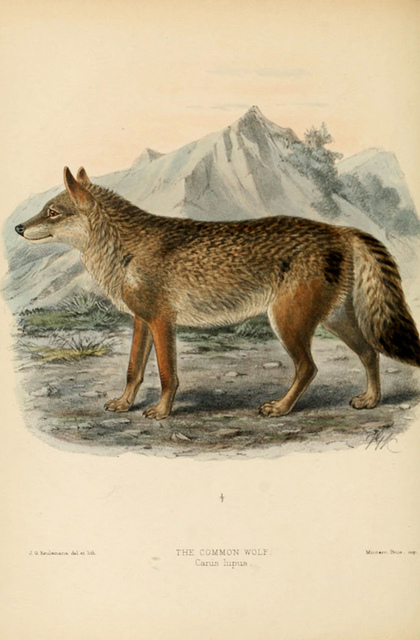
\includegraphics[width= \textwidth]{illustration_images/alleles_genotypes/grey_wolf/5988399184_0c36a8e51c_z.jpg}
\end{center}
\caption{Grey wolf ({\it Canis lupus}). \BHLNC{Dogs, jackals, wolves,
    and foxes: a monograph of the Canidae. 1890. y J.G. Keulemans}{https://www.biodiversitylibrary.org/page/17002968\#page/58/mode/1up}{University of Toronto - Gerstein Science Information Centre}} \label{fig:Grey_wolf}
\end{marginfigure}
They were extirpated in the wild during the mid-1900s due to hunting, and the remaining five Mexican wolves in the wild were captured to start a breeding program. \citet{vonHoldt:11} estimated the current-day, average expected heterozygosity to be $0.18$, based on allele frequencies at over forty thousand SNPs. However, the average Mexican wolf individual was only observed to be heterozygous at $12\%$ of these SNPs. Therefore, the average inbreeding coefficient for the Mexican wolf is $F = 1 -\nicefrac{0.12}{0.18}$, i.e. $\sim 33 \%$ of a lobo's genome is homozygous due to recent inbreeding in their pedigree.

%{\bf Q}\arabic{Question} \refstepcounter{Question}

%==Phenotypic resemblance between relatives ==
%<source-file filename="Quantative_traits.tex" display="Quantative_traits.wrapped.latexml.xhtml">

%==Phenotypic resemblance between relatives ==
%<source-file filename="Quantative_traits.tex" display="Quantative_traits.wrapped.latexml.xhtml">

  \paragraph{Genomic blocks of homozygosity due to inbreeding.}

As we saw above, close relatives are expected to share alleles IBD in
large genomic blocks. Thus, when related individuals mate and transmit
alleles to an inbred offspring, they transmit these alleles in big
blocks through meiosis. An example, lets return to the case of our
hypothetical first cousins from Figure
\ref{fig:IBD_cousins_chr_cartoon}. If this pair of individuals had a
child, one possible pattern of genetic transmission is shown in Figure
\ref{fig:kid_first_cousins}. The child has inherited the red stretch
of chromosome via two different routes through their predigree from
the grandparents. This is an example of an autozygous
segment, where the child is homozygous by descent at all of the loci in this
red region.
  \begin{figure}
  \begin{center}
    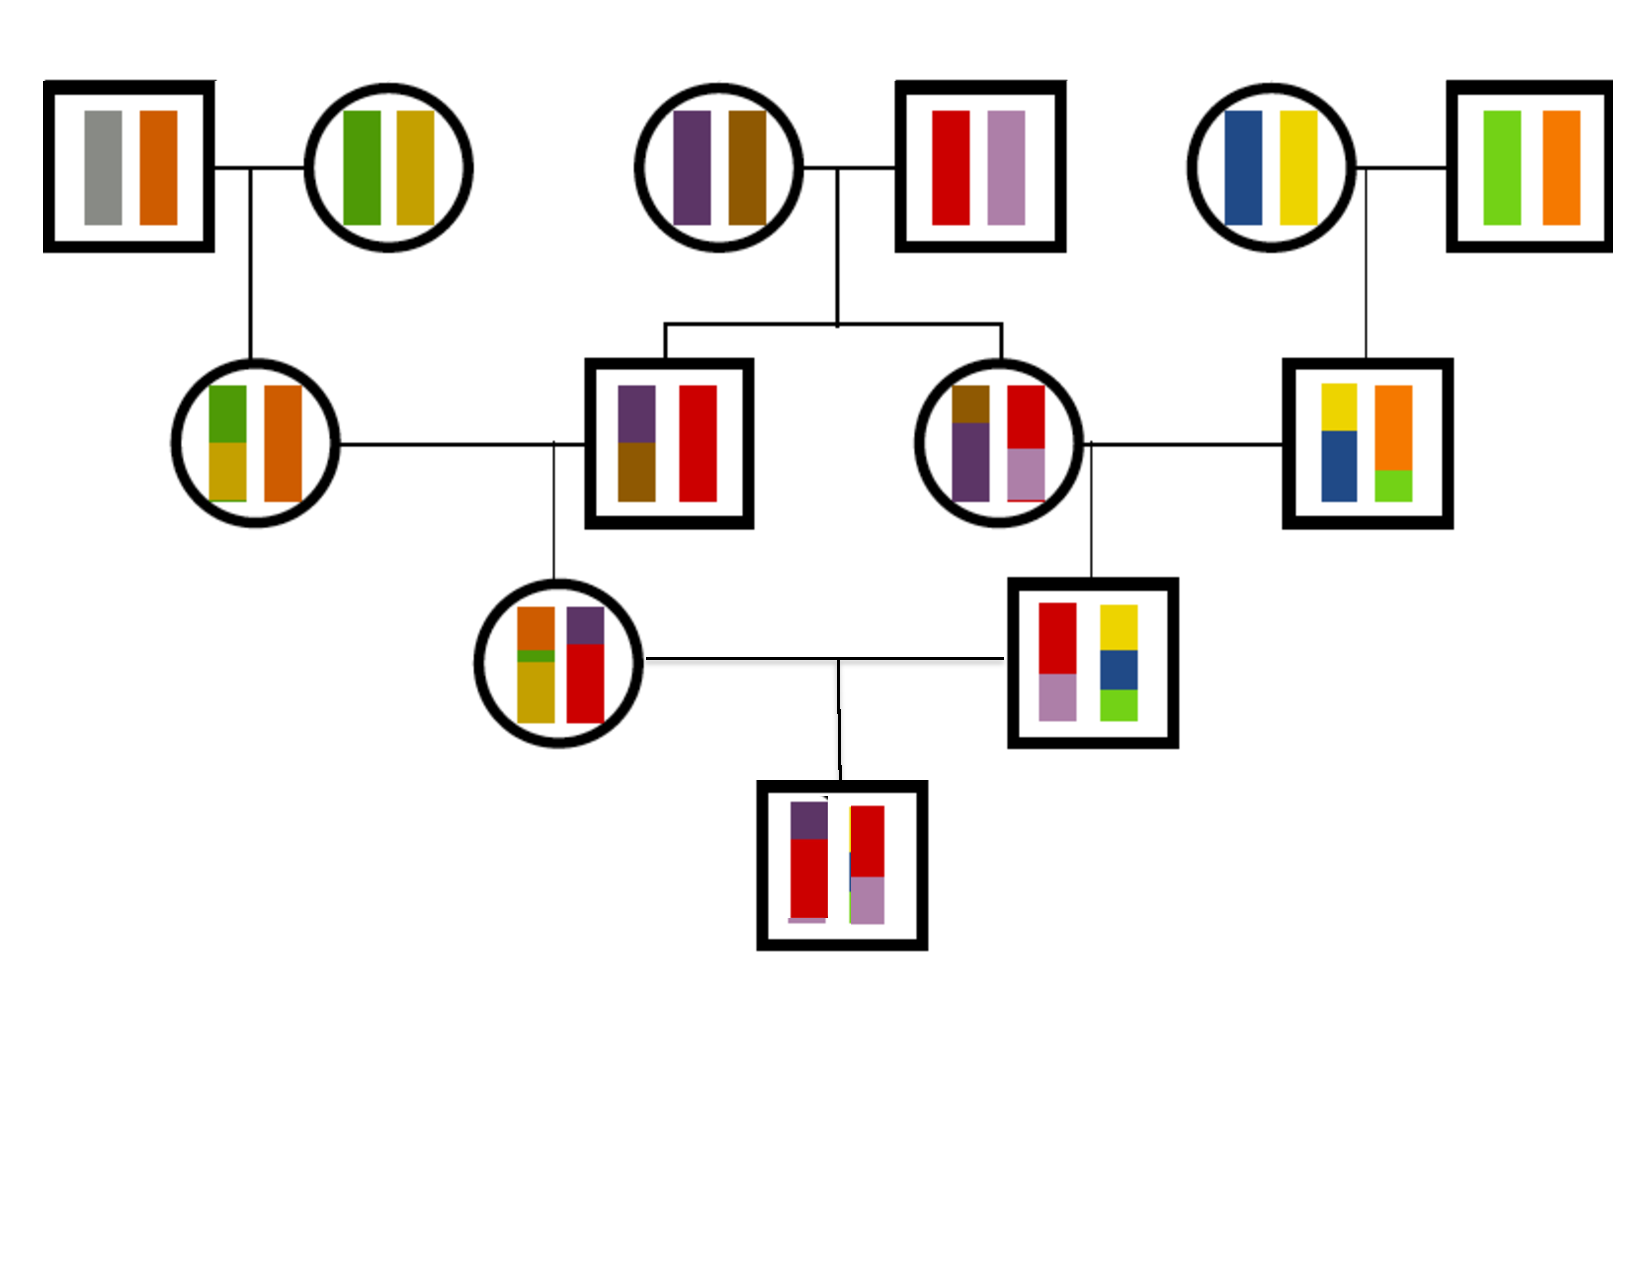
\includegraphics[width= 0.75 \textwidth]{figures/sharing_relatives/first_cousin_offspring.pdf}
\end{center}
\caption{A pedigree showing the offspring of first cousins. The
  chromosomes of their great-grandparents are coloured different colours
so their transmission can be tracked. The child is homozygous by
descent (HBD) for a section of the red chromosome.} \label{fig:kid_first_cousins}
\end{figure}
The inbreeding coefficient of the child sets the proportion of their
genome that will be in these autozygous segments. For example, a child
of first full cousins is expected to have $1/16$ of their
genome in these segments.
The more distant the loop in the pedigree, the more meioses that
chromosomes have been through and the shorter individual blocks will be. A
child of first cousins will have longer blocks than a child of second
cousins, for example.

Individuals with multiple inbreeding loops in their family tree can
have a high inbreeding coefficient due to
the combined effect of many small blocks of autozygosity. For example, Charles II had
an inbreeding coefficient that is equivalent to that of the child of
full-sibs, with a quarter of his genome expected to homozygous by
descent, but this would be made up of many shorter blocks.
%With multiple rounds of inbreeding individuals can

We can hope to detect these blocks by looking for unusually long
genomic runs of homozygosity (ROH) sites in an individual's genome. One way to
estimate an individual's inbreeding coefficient is then to total up
the proportion of an individual's genome that falls in such ROH
regions. This estimate is called $F_{ROH}$.

\graham{update to use figs from G3 Sam's article, and collapse to
  single ref.}
An example of using $F_{ROH}$ to study inbreeding comes from the work of
\citet{sams2018fine}, who identified runs of homozygosity in 2,500 dogs,
ranging from 500kb up to many megabases.
  \begin{figure}
  \begin{center}
    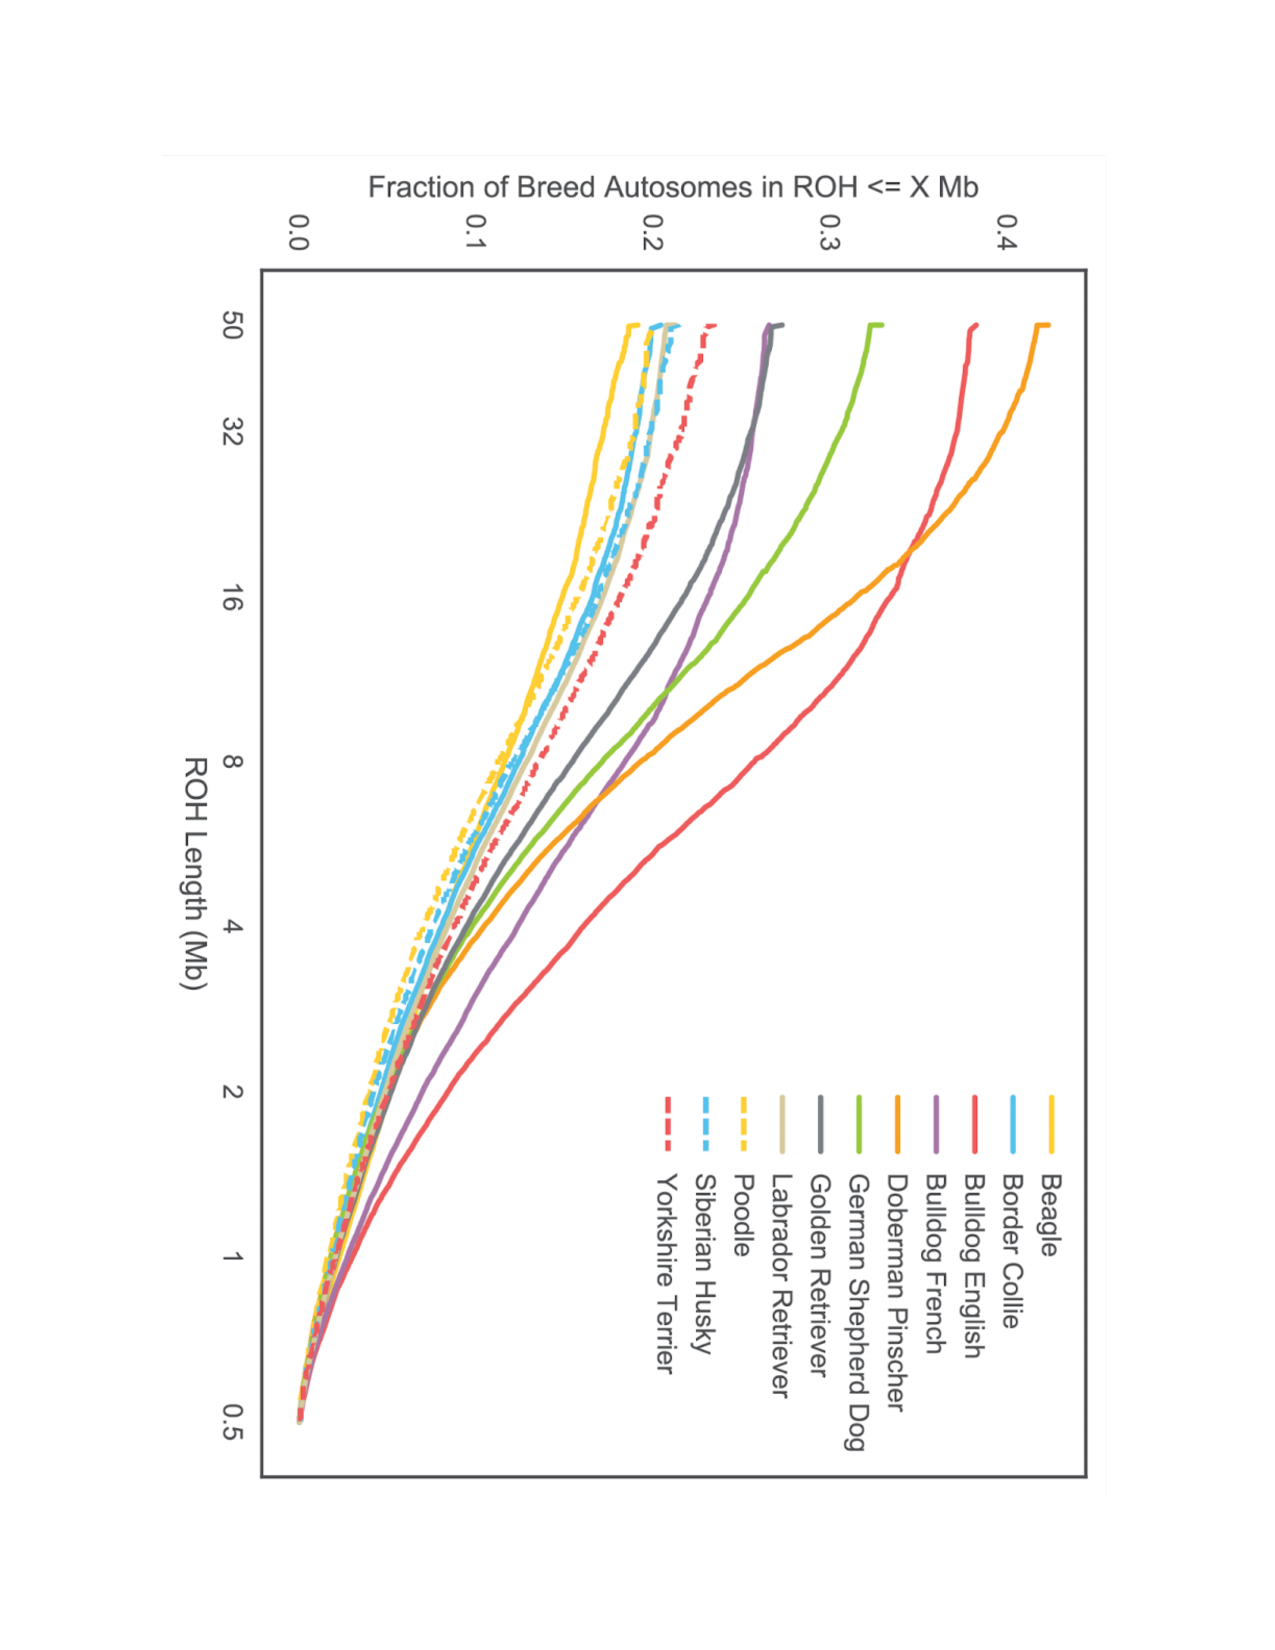
\includegraphics[width= \textwidth]{figures/sharing_relatives/dogs_FROH.pdf}
\end{center}
\caption{The distribution  of $F_{ROH}$ of individuals from various
  dog breeds from \citet{Sams:18}, \PLOSccBY.} \label{fig:dog_FOH}
\end{figure}
Figure
\ref{fig:dog_FOH} shows the distribution of $F_{ROH}$ of individuals in each dog
breed for the X and autosome. In Figure \ref{fig:dog_FOH_dist} this is
broken down by the length of ROH segments.
%JRI: No text reference to this figure. Why show a bulldog and not a mix of dog breeds?

  \begin{marginfigure}[-1cm]
  \begin{center}
    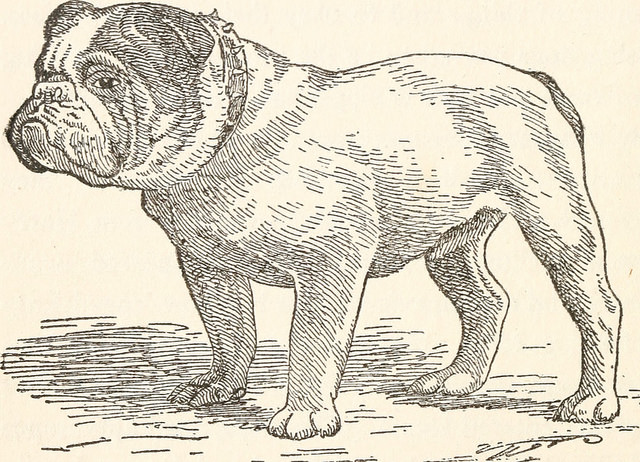
\includegraphics[width=
    \textwidth]{illustration_images/alleles_genotypes/english_bulldog/14752595581_4330377c97_z.jpg}
\end{center}
\caption{English bulldog. The dogs of Boytown. 1918.  Dyer, W. A.} \label{fig:bulldog}
\end{marginfigure}

Dog breeds have been subject
to intense breeding that has resulted in high levels of inbreeding. Of the population samples examined, Doberman Pinschers have the highest levels of their genome in runs of
homozygosity ($F_{ROH}$), somewhat higher than English bulldogs. In \ref{fig:dog_FOH_dist} we can see that English bulldogs have more short ROH than Doberman Pinschers, but that Doberman Pinschers have more of their genome in very large ROH ($>16 Mb$). This suggests that English bulldogs have had long history of inbreeding but that Doberman Pinschers have a lot of recent inbreeding in their history.

  \begin{figure}
  \begin{center}
    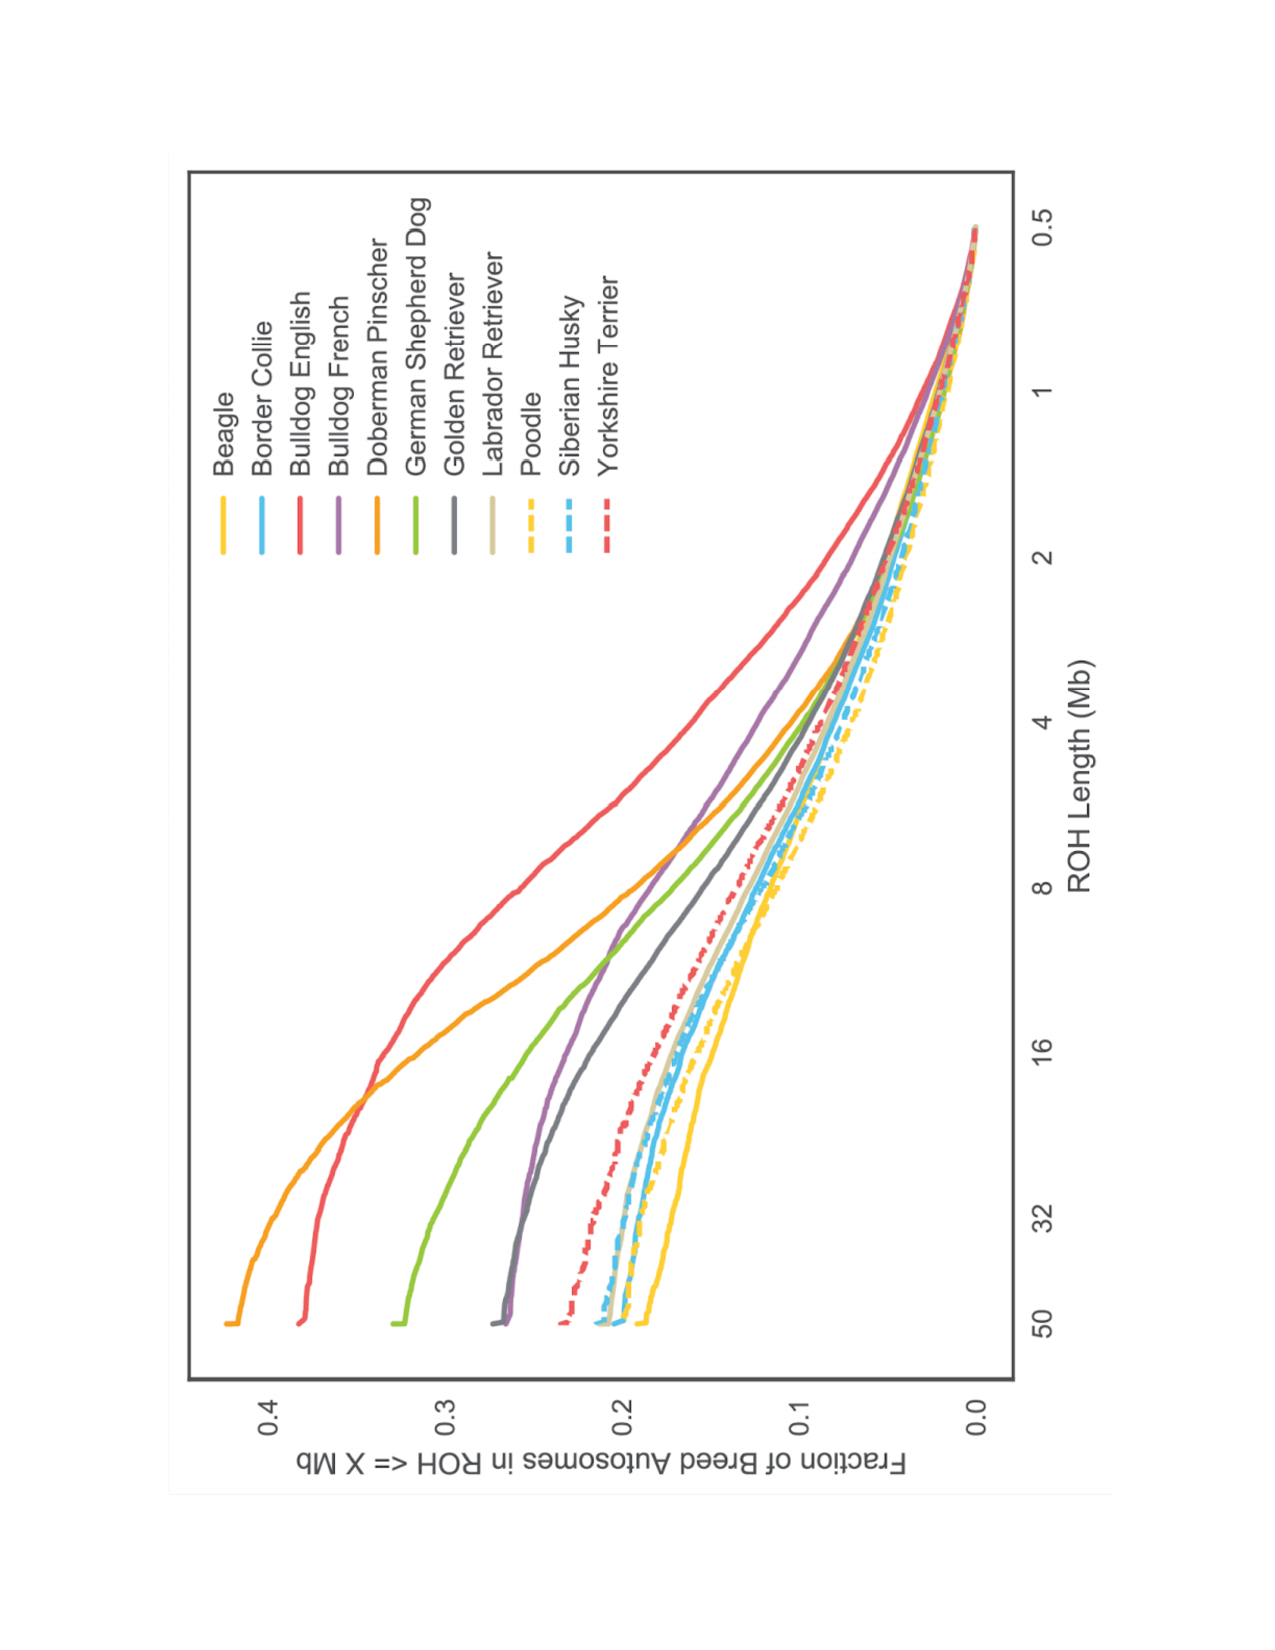
\includegraphics[width= \textwidth]{figures/sharing_relatives/dog_FROH_dist.pdf}
\end{center}
\caption{Cumulative density of ROH length, measured in megabases (Mb) from \citet{Sams:18} for various
  dog breeds (\PLOSccBY). Note that longer lengths of ROH are on the left of the plot.} \label{fig:dog_FOH_dist}
\end{figure}
